\documentclass{article}
%Usepackages
\usepackage{adjustbox, amsmath, amssymb, amsthm, blindtext, bm, bbm, dblfloatfix, esint, fancyhdr, float, graphicx, letltxmacro, marginnote, mathtools, subcaption, xcolor, titlesec, esint}
\usepackage{amssymb}
\usepackage[font={small, it}]{caption}
\usepackage{amsmath}
%\usepackage{floatrow}
\usepackage{times}
\usepackage{ stmaryrd }
\usepackage{amsthm}
\usepackage{xcolor}
\usepackage{mathrsfs}
\usepackage[colorlinks = true,
            linkcolor = black,
            urlcolor  = blue,
            citecolor = black,
            anchorcolor = blue]{hyperref}
% \usepackage[mathscr]{euscript}
\usepackage{mathrsfs}
\usepackage{wasysym}
%\usepackage{pxfonts}
\usepackage[letterpaper, portrait, margin=1in]{geometry}
\usepackage{graphicx}
\usepackage{tikz}
\usepackage{tikz-3dplot}
\usepackage{pgfplots}
\usetikzlibrary{decorations.pathmorphing,patterns}
\usepackage{lipsum}
\usepackage{float}
\usepackage{subcaption}
\usepackage[object=vectorian]{pgfornament}
\usepackage{mwe}
\usepackage{bigints}
\usepackage{titlesec}
\usepackage{halloweenmath}
\setcounter{secnumdepth}{4}
\titleformat{\paragraph}
{\normalfont\normalsize\bfseries}{\theparagraph}{1em}{}
\titlespacing*{\paragraph}
{0pt}{3.25ex plus 1ex minus .2ex}{1.5ex plus .2ex}
\usepackage{mathtools}
\usepackage{pgfplots}
\pgfplotsset{compat=1.15}
\usepackage{lastpage}
\usepackage{enumitem}
\usepackage{tensor}
\usepackage{mathtools}
\usepackage{fancyhdr} 
    \pagestyle{fancy}
    \fancyhf{}
    \rhead{ Page \thepage \  of \pageref{LastPage}}
    \lhead{MATH1410 Final Project}
\usepackage{setspace}
%\usepackage{tikz}
\usetikzlibrary{hobby}

\usepackage{pst-node}

\usepackage{tikz-cd}

% \makeatletter
% \renewcommand\@endtheorem{\vvv@endmarker\endtrivlist\@endpefalse}
% \newcommand\vvv@endmarker{%
%   {\unskip\nobreak\hfil\penalty50
%   \hskip2em\vadjust{}\nobreak\hfil\openbox
%   \parfillskip=0pt \finalhyphendemerits=0 \par
%   \penalty 10000 \parskip=0pt\noindent}\ignorespaces}
% \makeatother

\theoremstyle{definition}

\newtheorem{theorem}{Theorem}[section]
\newtheorem{definition}[theorem]{Definition}
\newtheorem{example}[theorem]{Example}
\newtheorem{lemma}[theorem]{Lemma}
\newtheorem{conjecture}[theorem]{Conjecture}
\newtheorem{exercise}[theorem]{Exercise}
\newtheorem{fact}[theorem]{Fact}
\newtheorem{claim}[theorem]{Claim}
\newtheorem{corollary}[theorem]{Corollary}

\newtheorem{idea}[theorem]{Idea}
\newtheorem{application}[theorem]{Application}
\newtheorem{remark}[theorem]{Remark}

\newtheorem{proposition}[theorem]{Proposition}
\newtheorem{question}[theorem]{Question}
\newenvironment{solution}
  {\renewcommand\qedsymbol{$\blacksquare$}\begin{proof}[Solution]}
  {\end{proof}}
\newenvironment{answer}
  {\begin{proof}[Answer]}
  {\end{proof}}
  
% \newenvironment{example}
%   {\pushQED{\qed}\renewcommand{\qedsymbol}{$\triangle$}\examplex}
%   {\popQED\endexamplex}




%%%%%%%%%%%%%%%%%%%%%%%%%%%%%

%Custom Commands
    \renewcommand\qedsymbol{$\blacksquare$}
    \newcommand{\Pcal}{\mathcal{P}}
    \newcommand{\ve}{\varepsilon}
    \newcommand{\Ocal}{\mathcal{O}}
    \newcommand{\Asf}{\textsf{A}}
    \newcommand{\al}{\alpha}
    \newcommand{\be}{\beta}
    \newcommand{\Nbb}{\mathbb{N}}
    \newcommand{\Si}{\Sigma}
    \newcommand{\Hbb}{\mathbb{H}}
    \DeclareMathOperator{\diag}{diag}
    \newcommand{\De}{\Delta}
    \newcommand{\Xcal}{\mathcal{X}}
    \newcommand{\si}{\sigma}
    \newcommand{\Ga}{\Gamma}
    \newcommand{\Cscr}{\mathscr{C}}
    \newcommand{\1}{\mathbf{1}}
    \newcommand{\Dcal}{\mathcal{D}}
    \newcommand{\Iscr}{\mathscr{I}}
    \newcommand{\Pbb}{\mathbb{P}}
    \newcommand{\B}{\mathbb{B}}
    \newcommand{\Dscr}{\mathscr{D}}
    \newcommand{\Nfrak}{\mathfrak{N}}
    \newcommand{\Efrak}{\mathfrak{E}}
    \DeclareMathOperator{\charp}{charpoly}
    \newcommand{\Csf}{\mathsf{C}}
    \newcommand{\rfrak}{\mathfrak{r}}
    \newcommand{\Sbb}{\mathbb{S}}
    \newcommand{\La}{\Lambda}
    \newcommand{\de}{\delta}
    \DeclareMathOperator{\inte}{int}
    \DeclareMathOperator{\ord}{ord}
    \newcommand{\set}{\mathsf{set}}
    \newcommand{\Bscr}{\mathscr{B}}
    \newcommand{\Zscr}{\mathscr{Z}}
    \newcommand{\ab}{\mathrm{ab}}
    \newcommand{\Xscr}{\mathscr{X}}
    \newcommand{\Escr}{\mathscr{E}}
    \newcommand{\Gscr}{\mathscr{G}}
    \DeclareMathOperator{\Sym}{Sym}
    \newcommand{\om}{\omega}
    \newcommand{\gfrak}{\mathfrak{g}}
    \newcommand{\hfrak}{\mathfrak{h}}
    \newcommand{\kfrak}{\mathfrak{k}}
    \newcommand{\Grp}{\mathsf{Grp}}
    \newcommand{\Ab}{\mathsf{Ab}}
    \newcommand{\xbar}{\bar{x}}
    \newcommand{\abar}{\bar{a}}
    \newcommand{\ybar}{\bar{y}}
    \DeclareMathOperator{\coker}{coker}
    \newcommand{\Modsf}{\mathsf{Mod}}
    \newcommand{\op}{\mathrm{op}}
    \newcommand{\Ring}{\mathsf{Ring}}
    \newcommand{\modsf}{\mathsf{mod}}
    \DeclareMathOperator{\Alt}{Alt}
    \newcommand{\Om}{\Omega}
    \newcommand{\ze}{\zeta}
    \newcommand{\Fcal}{\mathcal{F}}
    \newcommand{\Oscr}{\mathscr{O}}
    \newcommand{\gl}{\mathfrak{gl}}
    \DeclareMathOperator{\Lie}{Lie}
    \DeclareMathOperator{\GL}{GL}
    \DeclareMathOperator{\SL}{SL}
    \DeclareMathOperator{\Vol}{Vol}
    \DeclareMathOperator{\Disc}{Disc}
    \DeclareMathOperator{\SO}{SO}
    \newcommand{\Xfrak}{\mathfrak{X}}
    \DeclareMathOperator{\id}{id}
    \DeclareMathOperator{\Int}{Int}
    \DeclareMathOperator{\End}{End}
    \DeclareMathOperator{\Aut}{Aut}
    \DeclareMathOperator{\stab}{stab}
    \DeclareMathOperator{\orb}{orb}
    \DeclareMathOperator{\grad}{grad}
    \DeclareMathOperator{\curl}{curl}
    \newcommand{\vp}{\varphi}
    \newcommand{\vt}{\vartheta}
    \DeclareMathOperator{\Gal}{Gal}
    \DeclareMathOperator{\rank}{rank}
    \DeclareMathOperator{\col}{col}
    \DeclareMathOperator{\Tame}{Tame}  
    \newcommand{\Yscr}{\mathscr{Y}}
    \newcommand{\Fbb}{\mathbb{F}}
    \newcommand{\Hcal}{\mathcal{H}}
    \newcommand{\arctanh}{\text{arctanh}}
    \newcommand{\pa}{\partial}
    \newcommand{\del}{\boldsymbol{\nabla}}
    \newcommand{\na}{\nabla}
    \newcommand{\Ycal}{\mathcal{Y}}
    \DeclareMathOperator{\spn}{span}
    \DeclareMathOperator{\Inn}{Inn}
    \DeclareMathOperator{\chara}{char}
    \newcommand{\lap}{\nabla^2}
    \newcommand{\Pfrak}{\mathfrak{P}}
    \newcommand{\mfrak}{\mathfrak{m}}
    \newcommand{\Fvec}{\mathbf{F}}
    \newcommand{\Mcal}{\mathcal{M}}
    \newcommand{\ellvec}{\boldsymbol{\ell}}
    \newcommand{\rvec}{\mathbf{r}}
    \DeclareMathOperator{\supp}{supp}
    \newcommand{\Abb}{\mathbb{A}}
    \newcommand{\svec}{\mathbf{s}}
    \newcommand{\VECT}{\mathsf{VECT}}
    \newcommand{\fs}{\vec{\sigma}}
    \newcommand{\bs}{\cev{\sigma}}
    \newcommand{\uvec}{\mathbf{u}}
    \newcommand{\iunit}{\boldsymbol{\hat{\i}}}
    \newcommand{\junit}{\boldsymbol{\hat{\j}}}
    \newcommand{\xunit}{\mathbf{\hat{x}}}
    \newcommand{\Char}{\text{char}}
    \newcommand{\kunit}{\mathbf{\hat{k}}}
    \newcommand{\theunit}{\boldsymbol{\hat{\theta}}}
    \newcommand{\pvec}{\mathbf{p}}
    \newcommand{\qvec}{\mathbf{q}}
    \newcommand{\Qcal}{\mathcal{Q}}
    \newcommand{\yvec}{\mathbf{y}}
    \newcommand{\xvec}{\mathbf{x}}
    \newcommand{\wvec}{\mathbf{w}}
    \newcommand{\bvec}{\mathbf{b}}
    \newcommand{\Ucal}{\mathcal{U}}
    \newcommand{\Ncal}{\mathcal{N}}
    \newcommand{\Scal}{\mathcal{S}}
    \newcommand{\Nscr}{\mathscr{N}}
    \newcommand{\da}{\dagger}
    \newcommand{\CT}{\mathrm{H}}
    \newcommand{\Sscr}{\mathscr{S}}
    \DeclareMathOperator{\lcm}{lcm}
    \newcommand{\evec}{\mathbf{e}}
    \newcommand{\Kscr}{\mathscr{K}}
    \newcommand{\ebold}{\boldsymbol{e}}
    \newcommand{\zvec}{\mathbf{z}}
    \newcommand{\vvec}{\mathbf{v}}
    \newcommand{\Tscr}{\mathscr{T}}
    \newcommand{\avec}{\mathbf{a}}
    \newcommand{\Avec}{\mathbf{A}}
    \newcommand{\Ivec}{\mathbf{I}}
    \newcommand{\ivec}{\mathbf{i}}
    \newcommand{\jvec}{\mathbf{j}}
    \newcommand{\kvec}{\mathbf{k}}
    \newcommand{\of}{\mathfrak{o}}
    \DeclareMathOperator{\Ot}{O}
    \DeclareMathOperator{\Sy}{S}
    \newcommand{\slf}{\mathfrak{sl}}
    \newcommand{\muvec}{\boldsymbol{\mu}}
    \newcommand{\Bvec}{\mathbf{B}}
    \newcommand{\Cvec}{\mathbf{C}}
    \newcommand{\eunit}{\mathbf{\hat{e}}}
    \newcommand{\vpunit}{\boldsymbol{\hat{\varphi}}}
    \newcommand{\zero}{\boldsymbol{0}}
    \newcommand{\tauvec}{\boldsymbol{\tau}}
    \newcommand{\runit}{\mathbf{\hat{r}}}
    \newcommand{\U}{\mathcal{U}}
    \newcommand{\Zbb}{\mathbb{Z}}
    \newcommand{\Bsf}{\mathsf{B}}
    \DeclareMathOperator{\G}{G}
    \newcommand{\gmat}{\textsf{g}}
    \newcommand{\Ccal}{\mathcal{C}}
    \newcommand{\SM}{\mathsf{SM}}
    \newcommand{\VB}{\mathsf{VB}}
    \newcommand{\Dsf}{\mathsf{D}}
    \newcommand{\Fscr}{\mathscr{F}}
    \DeclareMathOperator{\Map}{Map}
    \DeclareMathOperator{\Frob}{Frob}
    \newcommand{\Imat}{\textsf{I}}
    \newcommand{\Rmat}{\textsf{R}}
    \DeclareMathOperator{\Frac}{Frac}
    \DeclareMathOperator{\Spec}{Spec}
    \DeclareMathOperator{\Emb}{Emb}
    \newcommand{\Kcal}{\mathcal{K}}
    \newcommand{\Wcal}{\mathcal{W}}
    \newcommand{\Lcal}{\mathcal{L}}
    \newcommand{\Tcal}{\mathcal{T}}
    \newcommand{\Ecal}{\mathcal{E}}
    \DeclareMathOperator{\im}{im}
    \newcommand{\Qbb}{\mathbb{Q}}
    \newcommand{\ga}{\gamma}
    \newcommand{\la}{\lambda}
    \newcommand{\RomanNumeralCaps}[1]
        {\MakeUppercase{\romannumeral #1}} 
    \newcommand{\dif}{\text{d}}
    \newcommand{\Rbb}{\mathbb{R}}
    \newcommand{\Tbb}{\mathbb{T}}
    \DeclareMathOperator{\Hom}{Hom}
    \DeclareMathOperator{\conv}{conv}
    \newcommand{\Vcat}{\mathsf{V}}
    \newcommand{\Gr}{\text{Gr}}
    \newcommand{\Bcal}{\mathcal{B}}
    \newcommand{\Acal}{\mathcal{A}}
    \newcommand{\pfrak}{\mathfrak{p}}
    \newcommand{\qfrak}{\mathfrak{q}}
    \newcommand{\Evec}{\mathbf{E}}
    \newcommand{\omvec}{\boldsymbol{\omega}}
    \newcommand{\alvec}{\boldsymbol{\alpha}}
    \newcommand{\gvec}{\mathbf{g}}
    \newcommand{\afrak}{\mathfrak{a}}
    \newcommand{\bfrak}{\mathfrak{b}}
    \newcommand{\Cbb}{\mathbb{C}}
    \newcommand{\gavec}{\boldsymbol{\gamma}}
    \newcommand{\Tvec}{\mathbf{T}}
    \newcommand{\Vscr}{\mathscr{V}}
    \newcommand{\Ascr}{\mathscr{A}}
    \newcommand{\Uscr}{\mathscr{U}}
    \newcommand{\Sfrak}{\mathfrak{S}}
    \DeclareMathOperator{\sgn}{sgn}
    \DeclareMathOperator{\vol}{vol}
    \newcommand{\Pscr}{\mathscr{P}}
    \newcommand{\Wscr}{\mathscr{W}}
    \newcommand{\bcdot}{\boldsymbol{\cdot}}
    \DeclareMathOperator{\tr}{tr}
    
    \newcommand{\sectionline}{
        \noindent
        \begin{center}
        {
        {{
        {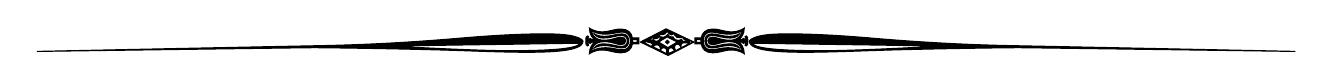
\begin{tikzpicture}
        \node  (C) at (0,0) {};
        \node (D) at (16,0) {};
        \path (C) to [ornament=89] (D);
        \end{tikzpicture}}}}}
        \end{center}
        }
    \newcommand{\sectionlineflip}{
        \noindent
        \begin{center}
        {
        {{
        {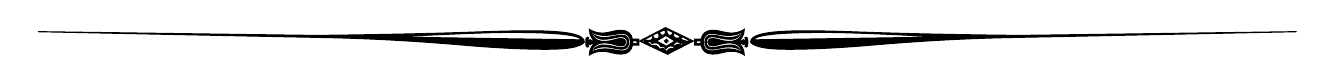
\begin{tikzpicture}
        \node  (C) at (0,0) {};
        \node (D) at (16,0) {};
        \path (D) to [ornament=89] (C);
        \end{tikzpicture}}}}} 
        \end{center}
        }
        

        
       
%%%%%%%%%%%%%%%%%%%%%%%%%%%%%%%
%Custom Symbols
\newcommand{\goodemptyset}[1]{%
\begin{tikzpicture}[#1]%
\draw (0,0) circle (0.1);%
\draw(-0.07,-0.14)--(0.07,0.14);
\end{tikzpicture}%
}

\newcommand{\es}{\raisebox{-1pt}{\goodemptyset{}}}


\makeatletter
\DeclareRobustCommand{\cev}[1]{%
  {\mathpalette\do@cev{#1}}%
}
\newcommand{\do@cev}[2]{%
  \vbox{\offinterlineskip
    \sbox\z@{$\m@th#1 x$}%
    \ialign{##\cr
      \hidewidth\reflectbox{$\m@th#1\vec{}\mkern4mu$}\hidewidth\cr
      \noalign{\kern-\ht\z@}
      $\m@th#1#2$\cr
    }%
  }%
}
\makeatother


\makeatletter
\DeclarePairedDelimiterX{\pmodx}[1]{(}{)}{{\operator@font mod}\mkern6mu#1}
\renewcommand{\pmod}{%
  \allowbreak
  \if@display\mkern18mu\else\mkern8mu\fi
  \pmodx
}
\makeatother
\DeclarePairedDelimiter\bra{\langle}{\rvert}
\DeclarePairedDelimiter\ket{\lvert}{\rangle}
\DeclarePairedDelimiterX\braket[2]{\langle}{\rangle}{#1 \delimsize\vert #2}

 
\makeatletter
\newcommand{\colim@}[2]{%
  \vtop{\m@th\ialign{##\cr
    \hfil$#1\operator@font colim$\hfil\cr
    \noalign{\nointerlineskip\kern1.5\ex@}#2\cr
    \noalign{\nointerlineskip\kern-\ex@}\cr}}%
}
\newcommand{\colim}{%
  \mathop{\mathpalette\colim@{\rightarrowfill@\scriptscriptstyle}}\nmlimits@
}
\renewcommand{\varinjlim}{%
  \mathop{\mathpalette\varlim@{\rightarrowfill@\scriptscriptstyle}}\nmlimits@
}
\renewcommand{\varprojlim}{%
  \mathop{\mathpalette\varlim@{\leftarrowfill@\scriptscriptstyle}}\nmlimits@
}


% %%%%%%%%%%%%%%%%%%%%%%%%%%%%%
% %Just arrows (cause normy arrows suck)
% \newcommand{\goodarrow}[1]{
% \begin{tikzpicture}[#1]
% \draw[-stealth] (0,0)--(0.4,0);
% \end{tikzpicture}
% }

% \renewcommand{\to}{\raisebox{2.4pt}{\hspace{0.08cm}\goodarrow{}\hspace{0.06cm}}}

% %%%%

% \newcommand{\goodtwoheadrightarrow}[1]{
% \begin{tikzpicture}[#1]
% \draw[->>, >=stealth] (0,0)--(0.4,0);
% \end{tikzpicture}
% }

% \renewcommand{\twoheadrightarrow}{\raisebox{2.4pt}{\hspace{0.08cm}\goodtwoheadrightarrow{}\hspace{0.06cm}}}

% %%%

% \newcommand{\goodhookrightarrow}[1]{
% \begin{tikzpicture}[#1]
% \draw[right hook-stealth] (0,0)--(0.4,0);
% \end{tikzpicture}
% }

% \renewcommand{\hookrightarrow}{\raisebox{2.3pt}{\hspace{0.08cm}\goodhookrightarrow{}\hspace{0.06cm}}}

% %%%

% \newcommand{\goodmapsto}[1]{
% \begin{tikzpicture}[#1]
% \draw[-stealth] (0,0)--(0.4,0);
% \draw[] (0,0.06)--(0,-0.06);
% \end{tikzpicture}
% }

% \renewcommand{\mapsto}{\raisebox{0pt}{\hspace{0.02cm}\goodmapsto{}\hspace{0.03cm}}}


% %%%%%%%%%%%%%%%%%%%%%%%%%%%%%

% \tikzcdset{arrow style=tikz, diagrams={>={stealth[round,length=4pt,width=4.5pt,inset=2.75pt]}}}






\renewcommand*\contentsname{Table of Content}

\title{Van Kampen's Theorem and the Wirtinger Presentation}
\author{Alice Foster, Mattie Ji}
\date{Updated: December 12th, 2021}

\begin{document}

\maketitle



\section*{Introduction:}
The ability to distinguish between ``different" knots is central to knot theory; therefore, throughout history, knot theorists have approached this classification problem in a variety of ways. Our Final Project aims to introduce a popular method of studying knot theory from the perspective of Algebraic Topology, using Van Kampen's theorem to calculate the fundamental group of the complement of knots.\\\\
We will begin by a brief introduction of mathematical knots and knot groups in Section $1$. We will then establish the notion of free groups, groups presentations, and other tools in Section $2$. We need these definitions to understand how to distinguish knots. We will discuss Van Kampen's Theorem in Section $3$, which employs free groups to describe how the fundamental groups of open subsets of a space can generate the fundamental group of the space. Finally, in Section $4$, we will use Van Kampen's Theorem to write a group presentation of a given knot, known as the \textit{Wirtlinger Presentation}. We use these presentations to distinguish knots.\\\\
This project assumes basic knowledge in Point-Set and Algebraic Topology, as well as Group Theory. This was drawn in part from Paul Armstrong's \textit{Basic Topology} \cite{armstrong_1983} and James Munkres's \textit{Topology} \cite{munkres2000topology}.

\tableofcontents

\newpage
\section{What is a knot?}
Knot theory is a centuries-old field of study. A knot in mathematics is much like a knot in the real world: a string looped around itself without being torn apart. In mathematics, we require the two ends of the string to be "glued" together. A knot is therefore like a tangled circle. We define a knot formally below.
\begin{definition}[Knot]
A \emph{knot} is an embedding of the circle, $S^1$, in $\mathbb{R}^3$.\\\\
We say $S^1$ is \emph{embedded} in $\mathbb{R}^3$ if there is an injective, continuous map $f:S^1 \rightarrow \mathbb{R}^3$ such that $f(S^1)$, a subspace of $\mathbb{R}^3$ with the subspace topology, is homeomorphic to $S^1$.
\end{definition}

\begin{remark}
Knots can be visualized in two-space with a \emph{knot diagram}. Knot diagrams show where the knot crosses over itself. Knots are named according to the number of crossings in their knot diagram. In the third example below, the knot crosses itself seven times. Since there are multiple knots with the same number of crossings, knots are assigned an arbitrary subscript. In this case it is 3. Hence the name $7_{3}$.
\end{remark}

The most simple example of a knot is the unknot, which is a loop without tangles.
\begin{figure}[H]
\centering
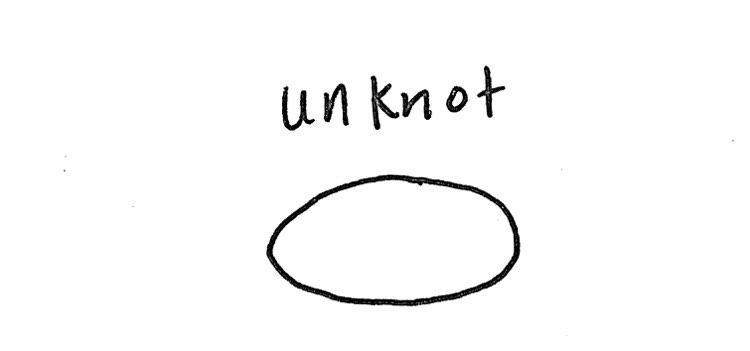
\includegraphics[scale=0.2]{figures/unknot.jpg}
\end{figure}

Another simple example is the trefoil knot.
\begin{figure}[H]
\centering
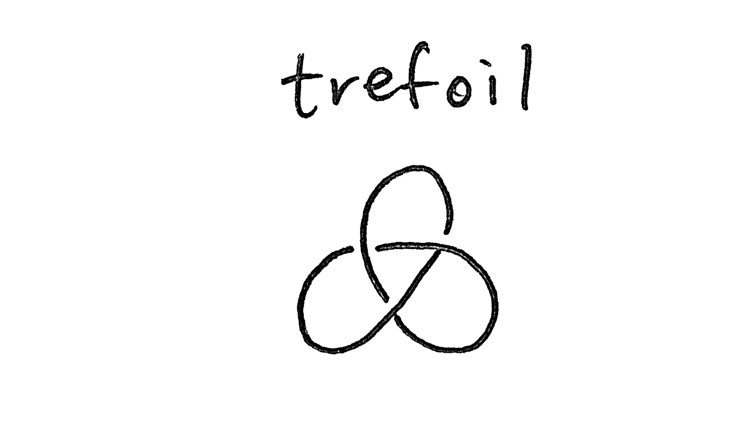
\includegraphics[scale=0.2]{figures/trefoil.jpg}
\end{figure}

Here is a more complicated knot:
\begin{figure}[H]
\centering
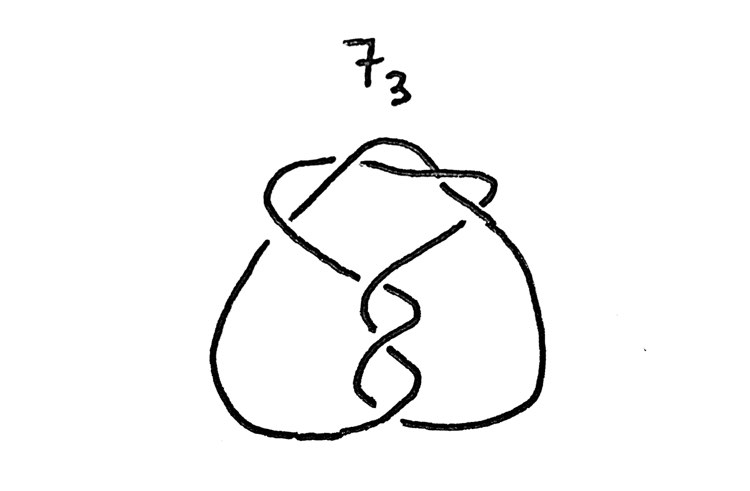
\includegraphics[scale=0.2]{figures/knot73.jpg}
\end{figure}

\noindent Now, how do we know if two knots are the same? We usually consider two spaces equivalent if they are homeomorphic. The spaces $K_1$ and $K_2$ of two knots are always homeomorphic; both spaces are homeomorphic to the circle. We must create a more meaningful definition of knot equivalence.

\noindent In general terms, two knots are equivalent if one can be deformed into the other without tearing it, eg, without passing it through itself. Formally,

\begin{definition}[Knot Equivalence]
Two knots $K_1$ and $K_2$ in $\mathbb{R}^3$ are \eph{equivalent} if there is a homeomorphism $f$ between $\mathbb{R}^3$ and itself such that $f(K_1) = K_2$.
\end{definition}

\noindent Now we introduce an object that will help us determine knot equivalence.
\begin{definition}[Knot Group]
The knot group of a knot $K$ is the fundamental group of $\mathbb{R}^3\setminus{K}$.
\end{definition}
\noindent The knot group is a knot invariant, meaning that equivalent knots have isomorphic knot groups. The contrapositive of this statement is that two knots are different if their knot groups are different. This means we can use knot groups to figure out if two knots are different.

\newpage
\section{Free Group and Group Presentations}
Much of this section was based on Paolo Aluffi's \textit{Algebra : Chapter 0} \cite{aluffi2021algebra}.\\\\
The idea of free groups arose from the question: given an arbitrary set A, what is the most ``efficient" way to construct a group, which we will call $F(A)$, from the set in the sense that there's as little amount of relations as possible (hence the name ``Free") in the constructed group based on the set A.\\\\
One can imagine that in this new F(A), each element would essentially correspond to a random combination of elements from the set A itself. Indeed, that's where the motivation for a free group arises from.
\begin{definition}[Letters] Let A be a set, and let $$A^{-1} = \{a^{-1} : a \in A\}$$ be the set of ``inverse symbols" of A, then we call the combined set $A \bigcup A^{-1}$ the letters of A.\\
\end{definition}
\begin{definition}[Word] A word w from A is a finitely written product of elements from $A\bigcup A^{-1}$, ie, a word of length n can be expressed as:
\[w = a_0a_1...a_n\]
for $a_i = b_i^{\pm 1}$ and $b_i \in A$\\\\
For example, if $A = \{a, b\}$, then $w = abaab^{-1}$ is a word of length 5.\\\\
The product of zero letters is also a word; it's called the empty word.\\\\
Note that since there's no group properties yet, the word $w_1 = bb^{-1}$ and the word $w_2 = aa^{-1}$ are two different words.\\
\end{definition}

\begin{definition}[Reduction] Given a word w from A, we define a reduction operation $r: W(A) \to W(A)$ to be the process where r finds the first occurrence of $a^{-1}a$ or $aa^{-1}$ for any $a \in A$ in w and removes that term from w. If the word w has no occurrences of $a^{-1}a$ or $aa^{-1}$ for any $a \in A$, then $r(w) = w$.\\\\
For example, if $A = \{a, b, c\}$, for the word $w = abcc^{-1}baa^{-1}$, then $r(w) = abbaa^{-1}$, and $r(r(w)) = abb$.\\
\end{definition}

\begin{definition}[Reduced Word]
Let w be a word of length n from the set A. Then we call $r^{\lfloor \frac{n}{2} \rfloor}(w)$ a reduced word.
\end{definition}
\noindent The main idea of a reduced word is to get rid of the only relation in a group that we know for sure of that when the letter and its inverse are adjacent to one another, they should ideally become the identity in our group construction. A reduced word is essentially a word where no said adjacency can occur.\\\\
Consequently, one can see that the definition given for the reduced word has no said adjacency because in any word of length n, there are at most $\lfloor \frac{n}{2} \rfloor$ occurrences of this adjacency, which would all be removed by r.\\

\begin{definition}[Free Group]
Let $F(A)$ be the set of all reduced words of A. Then one can verify that $F(A)$ is a group under the operation {\bf concatenation-reduction} where, for any $w, v \in F(A)$, $w = a_0a_1.._a_n$, $v = b_0b_1...b_n$:
\[w \cdot_{F(A)} v = r(wv)\]
where the word $wv = a_0a_1..a_nb_0b_1...b_n$.\\\\
We call $F(A)$ with the operation given the {\bf free group} of A.\\
\end{definition}

\begin{example}
There are some common examples of free groups you may be familiar with:
\begin{enumerate}
    \item $F(\O)$ is the trivial group.
    \item $F(\{a\})$ consists of $\{..., a^{-1}a^{-1}, a^{-1}, \{\}, a, aa, ...\}$ is isomorphic to $\mathbb{Z}$.
    \item If A is a finite set of cardinality n, then we call $F(A)$ the free group of rank n.
\end{enumerate}
\end{example}

\noindent It turns out that every group G can be expressed as a quotient of a free group (just consider $F(G)$ and first isomorphism theorem), but often times one can express a group as a quotient of a free group generated with elements less than G. So in this senese, we can express every group G in terms of a sometimes simpler presentation of G in relations to a free group. This is also motivates the next definition below.
\begin{definition}[Group Presentation] Let A be some set and $R \subset F(A)$ with normal closure N in $F(A)$, then the natural homomorphism $\phi: F(A) \to G$ that evaluates each word as a multiplication of its letters in G, is clearly surjective and has kernel $ker(\phi) = N$.\\\\
Then we write $G = \frac{F(A)}{ker(\phi)}$ and denote its presentation as $G = \langle A | R \rangle = \langle A | r_1 = r_2 = ... = r_n = e \rangle$ for $r_i \in R$.\\\\
A is called the {\bf generators} of G, and R is called the ${\bf relations}$ of G.
\end{definition}
\noindent Since every group is the quotient of a free group, every group has a group presentation!
\begin{example} There are some familiar examples of presentations whose properties you may have seen already.
\begin{enumerate}
    \item Let $A = \{a_1, ..., a_n\}$, then $F(A) = \langle a_1, ..., a_n |\ \rangle$, that is, a free group has no relations.
    \item Let $n \in \mathbb{N}$, then $\mathbb{Z}/n\mathbb{Z} \cong \langle x\ |\ x^n = e\rangle$
    \item Let $D_{2n}$ be the dihedral group of the regular $n-gon$, then
    \[D_{2n} \cong \langle r,f\ |\ r^n = e, f^2 = e, frf = r^{-1}\rangle\]
    \item $\mathbb{Z} \times \mathbb{Z} \cong \langle a,b\ |\ ab = ba\rangle$
\end{enumerate}
\end{example}

\noindent With the idea of group presentations, one might ask if there's some way of combining group presentations together. And indeed, that's the core idea of a {\bf Free Product}.

\begin{definition}[Free Product] Let G, H be groups with presentations $G = \langle A_G | R_G \rangle$ and $H = \langle A_H | R_H \rangle$, then we define the free product ($*$) of G and H to be:
\[G * H = \langle A_G \cup A_H | R_G \cup R_H \rangle\]
\end{definition}

\begin{example}
There are several examples of free products that aligns with our pre-existing beliefs.
\begin{enumerate}
    \item {\bf (Free Product of Free Groups)} Let $F(A) = \langle a_1, ..., a_n\ |\ \rangle$, $F(B) = \langle b_1, ..., b_m\ |\ \rangle$, then $F(A)*F(B) = \langle a_1, ..., a_n, b_1, ..., b_n\ |\ \rangle$ is a free group of rank $m+n$.
    \item Let $\mathbb{Z}/n\mathbb{Z} \cong \langle x\ |\ x^n = e\rangle$ and $\mathbb{Z}/m\mathbb{Z} \cong \langle y\ |\ y^m = e\rangle$, then 
    \[\mathbb{Z}/n\mathbb{Z}*\mathbb{Z}/m\mathbb{Z} = \langle x, y\ |\ x^n = e, y^m = e\rangle\]
\end{enumerate}
\end{example}

\begin{definition}[Free Product with Amalgamation] Let G, H, A be arbitrary groups with presentatons $G = \langle A_G | R_G \rangle$, $H = \langle A_H | R_H \rangle$, $A = \langle B | R_A \rangle$ with two injective homomorphisms $f_1: A \to G$ and $f_2: A \to H$, let
\[R = \{f_1(a)f_2(a)^{-1}\ |\ a \in B\}\]
Then we call the free product of G and H with amalgamation A:
\[G *_A H = \{A_G \cup A_H | R_G \cup R_H \cup R\}\]

\noindent The diagram below shows how $A$, $G$, and $H$ relate to each other by the maps $f_1$ and $f_2$ and produce the free product with amalgamation $A$.
% https://q.uiver.app/?q=WzAsNCxbMCwxLCJBIl0sWzEsMCwiRyJdLFsxLDIsIkgiXSxbMiwxLCJHICpfQSBIIl0sWzAsMSwiZl8xIl0sWzAsMiwiZl8yIiwyXSxbMiwzLCIiLDIseyJzdHlsZSI6eyJib2R5Ijp7Im5hbWUiOiJkYXNoZWQifX19XSxbMSwzLCIiLDAseyJzdHlsZSI6eyJib2R5Ijp7Im5hbWUiOiJkYXNoZWQifX19XV0=
\[\begin{tikzcd}
	& G \\
	A && {G *_A H} \\
	& H
	\arrow["{f_1}", from=2-1, to=1-2]
	\arrow["{f_2}"', from=2-1, to=3-2]
	\arrow[dashed, from=3-2, to=2-3]
	\arrow[dashed, from=1-2, to=2-3]
\end{tikzcd}\]

\end{definition}

\begin{example}
Consider the free groups $G = \mathbb{Z}_{4} = \langle a | a^4\rangle$, $H = \mathbb{Z}_{6} = \langle b | b^6 \rangle$, and $A = \mathbb{Z}_{2} = \langle c | c^2 \rangle$.\\\\
To find the free product of $G$ and $H$ with amalgamation $A$, we first ask how we can define injective homomorphisms $f_1: A \to G$ and $f_2: A \to H$. The subgroup of $G$ that is homomorphic to $A$ is $\langle e, a^2\rangle$. The subgroup of $H$ homomorphic to $A$ is $\langle e, b^3 \rangle$. So we define $f_1$ such that $f_1(c) = a^2$ and $f_2$ such that $f_2(c) = b^3$. We want our free product to have $f_1(c) = f_2(c)$ for all $c \in A$, so we let $ R = \{a^2b^{-3}\}$ and obtain the free product of $G$ and $H$ with amalgamation $A$: \[G *_A H = \langle a,b | a^4 = e,b^6=e,a^2b^{-3}=e \rangle\]
\end{example}

\newpage
\section{What is Van Kampen's Theorem?}
\begin{theorem} Let X be the union of two open and path-connected topological spaces A and B, and $A \cap B$ is path-connected and non-empty. Then we have that:
\[\pi_1(X) \cong \pi_1(A) *_{\pi_1(A \cap B)} \pi_1(B)\]
where $\pi_1(X)$ is isomorphic to the free product of $\pi_1(A)$ and $\pi_1(B)$ with amalgamation of the $\pi_1(A \bigcap B)$ with injective homomorphisms $f_i: \pi_1(A \cap B) \to \pi_1(A)$ and $f_j: \pi_1(A \cap B) \to \pi_1(B)$ being the homomorphisms induced by the inclusion maps $i: A \cap B \to A$ and $j: A \cap B \to B$ respectively.
\end{theorem}
\noindent A lot of times calculating fundamental groups of certain spaces can feel like a hyper-case-specific solution for each space given. However, the use of Van Kampen's Theorem can help to simplify a lot of complications that may arise in more elementary methods.\\\\
We will run a few examples to give the reader a feel of the utility brought forth by Van Kampen's Theorem.
\begin{example}[Union of two Simply Connected Spaces]
Let X be the union of two open and path-connected topological spaces A and B, if A and B are both simply-connected, and $A \cap B$ is path-connected and non-empty, then X is also simply connected.
\begin{proof}
Since A and B are simply connected, we know their fundamental groups have presentations:
\[\pi_1(A) = \langle \O\ |\ \O\rangle\]
\[\pi_1(B) = \langle \O\ |\ \O\rangle\]
\[\pi_1(A \bigcap B) = \langle a_1, ..., a_n\ |\ r_1, ..., r_m\rangle\]
Then by Van Kampen's Theorem, we know that:
\[\pi_1(X) = \langle \O \cup \O\ |\ .....\rangle\]
Regardless of how many relations $\pi_1(A \bigcap B)$ gives to $\pi_1(X)$, we know that the generators of $$\pi_1(X) = \pi_1(A) *_{\pi_1(A \cap B)} \pi_1(B)$$ has 0 generators. So $\pi_1(X)$ is the trivial group,\\\\
Since X is path-connected, and $\pi_1(X)$ is trivial, X is simply connected.
\end{proof}
\end{example}

\begin{example}[Simply Connected Intersection]
Let X be the union of two open and path-connected topological spaces A and B, if $A \cap B$ is simply connected, then $\pi_1(X) \cong \pi_1(A)*\pi_1(B)$
\begin{proof}
$\pi_1(A), \pi_(B)$ have presentations
\[\pi_1(A) = \langle A_G\ |\ A_R\rangle\]
\[\pi_1(B) = \langle B_G\ |\ B_R\rangle\]
Since $A \bigcap B$ is simply connected, 
\[\pi_1(A \cap B) = \langle \O\ |\ \O\rangle\]
Then by Van Kampen's Theorem, we know that:
\[\pi_1(X) = \langle A_G \cup B_G\ |\ A_R \cup B_R \cup \O\rangle\]
which is the free product of $\pi_1(A)$ and $\pi_1(B)$.
\end{proof}
\end{example}

\begin{example}[A plane with $n$ points removed]
Let S be $\mathbb{R}^2$ with $n$ points removed, then we claim that $\pi_1(S)$ is the free group of rank $n$.
\begin{proof}
We will prove this with induction.\\\\
When $n = 0$, we know $S = \mathbb{R}^2$ and $\pi_1(\mathbb{R}^2)$ is the trivial group, which is the free group of rank 0\\\\
When $n = 1$, we know S deformation retracts to $S^1$, and $\pi_1(S^1) \cong \mathbb{Z}$, which is the free group of rank 1.\\\\
Now suppose our inductive hypothesis is true until $n = k$, then we wish to prove with $\mathbb{R}^2$ with $k+1$ points removed has fundamental group being the free group of rank $k+1$. Indeed, we can draw a line L through S such that there are $r$ points on one side of the line and $(k + 1) - r$ points on the opposite side. We can choose L such that $r$ is at least 1.\\\\
Now consider open, path-connected set U, V such that U covers the side of L with r points and over the line L by a distance of less than $\epsilon$ with respect to L, and V covers the side of L with $(k+1)-r$ points and over the line L by a distance of less than $\epsilon$ with respect to L. Furthermore, $\epsilon$ can be chosen such that there are no punctures in $U \bigcap V$.\\\\
By our inductive hypothesis and the fact that it holds on $n = 0, 1$. we know that $U$ homotopies to a plane with $r$ punctures, so $\pi_1(U)$ is a free group of rank r, $V$ homotopies to a plane with $(k+1)-r$ punctures, so $\pi_1(V)$ is a free group of rank $(k+1)-r$, and finally $U \bigcap V$ homotopes to a plane with 0 punctures, so $\pi_1(U \cap V)$ is trivial and $U \cap V$ is simply connected.\\\\
Thus, by Van Kampen and Example 3.3, $\pi_1(S)$ is just the free product of $\pi_1(U)$ and $\pi_1(V)$, so $\pi_1(S)$ is just the free group of rank $r + (k+1) - r = k+1$. This concludes the inductive steps.\\\\
Thus, the fundamental group of $\Rbb^2$ with $n$ punctures is exactly the free group of rank $n$.
\end{proof}
\end{example}

\newpage
\section{Applications of Van Kampen's Theorem in Knot Theory}
This section was learned and adapted from Rolfsen's book ``Knots and Links" \cite{rolfsen_2004}.\\\\
So far, we have seen some applicability of Van Kampen's Theorem in the calculation of fundamental groups. However, it seems fairly limited in a case-by-case scenario because one would need to find the specific subspaces they are looking for with a given space when using Van Kampen's Theorem.\\\\
Therefore, one might ask if there's a more general procedure to calculate the knot group of a given knot so that we could skip the laborious work of calculating the knot group on a case-by-case basis.\\\\
The answer is yes! And it comes from what's known as the {\bf ``Wirtinger Presentation"}.
\begin{definition}
Given an arbitrary knot diagram, we divide the knot into $n$ arcs. An arc is a section of the knot between two crossings. We assign the knot an orientation and label each arc $a_i$, where $a_i$ is connected to $a_{i - 1\ (mod\ n)}$ before and $a_{i + 1\ (mod\ n)}$ after.\\\\
For each $a_i$,  we establish conventions for the direction of a loop $s_i$ around arc $a_i$. $s_i$ is a loop from basepoint $(0, 0, 1)$ down and under $a_i$ and back to the basepoint. We have the orientation of $s_i$ go from ``right to left" below arc a. We illustrate the orientation and structure of $s$ with respect to $a$ in Figures 1 and 2:

\begin{figure}[h!]
		\centering
		\captionsetup{width=.75\linewidth}
		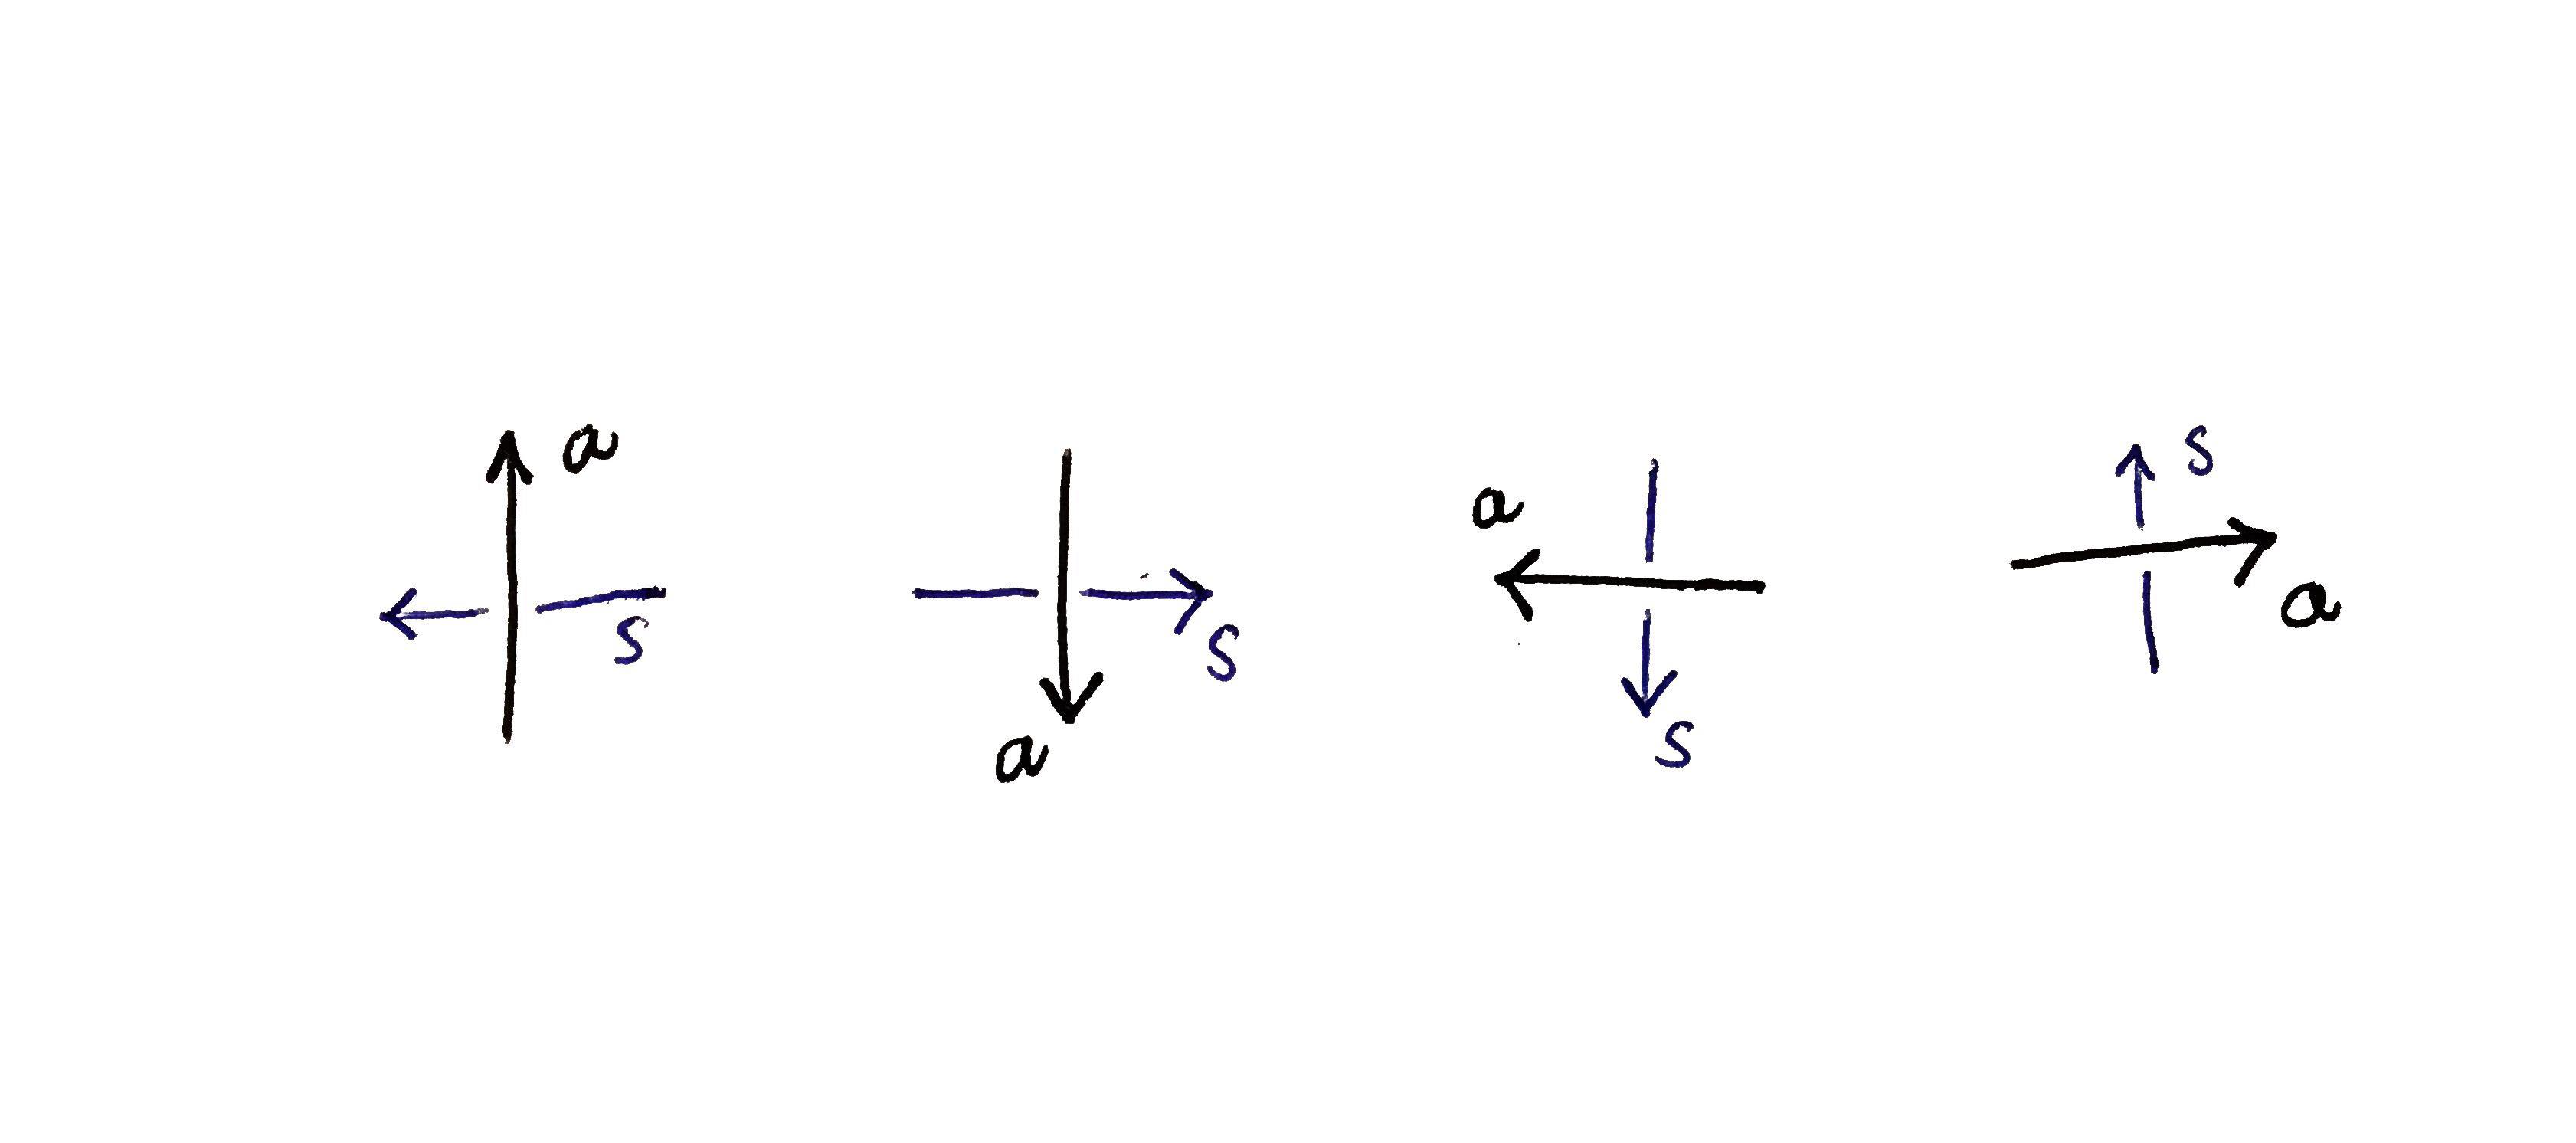
\includegraphics[width=6in]{figures/orientations.png}
		\caption{Here we show the direction of loop s around arc a.}
		\label{fig:rtinstability}
\end{figure}

\begin{figure}[h!]
	\centering
	\captionsetup{width=.75\linewidth}
	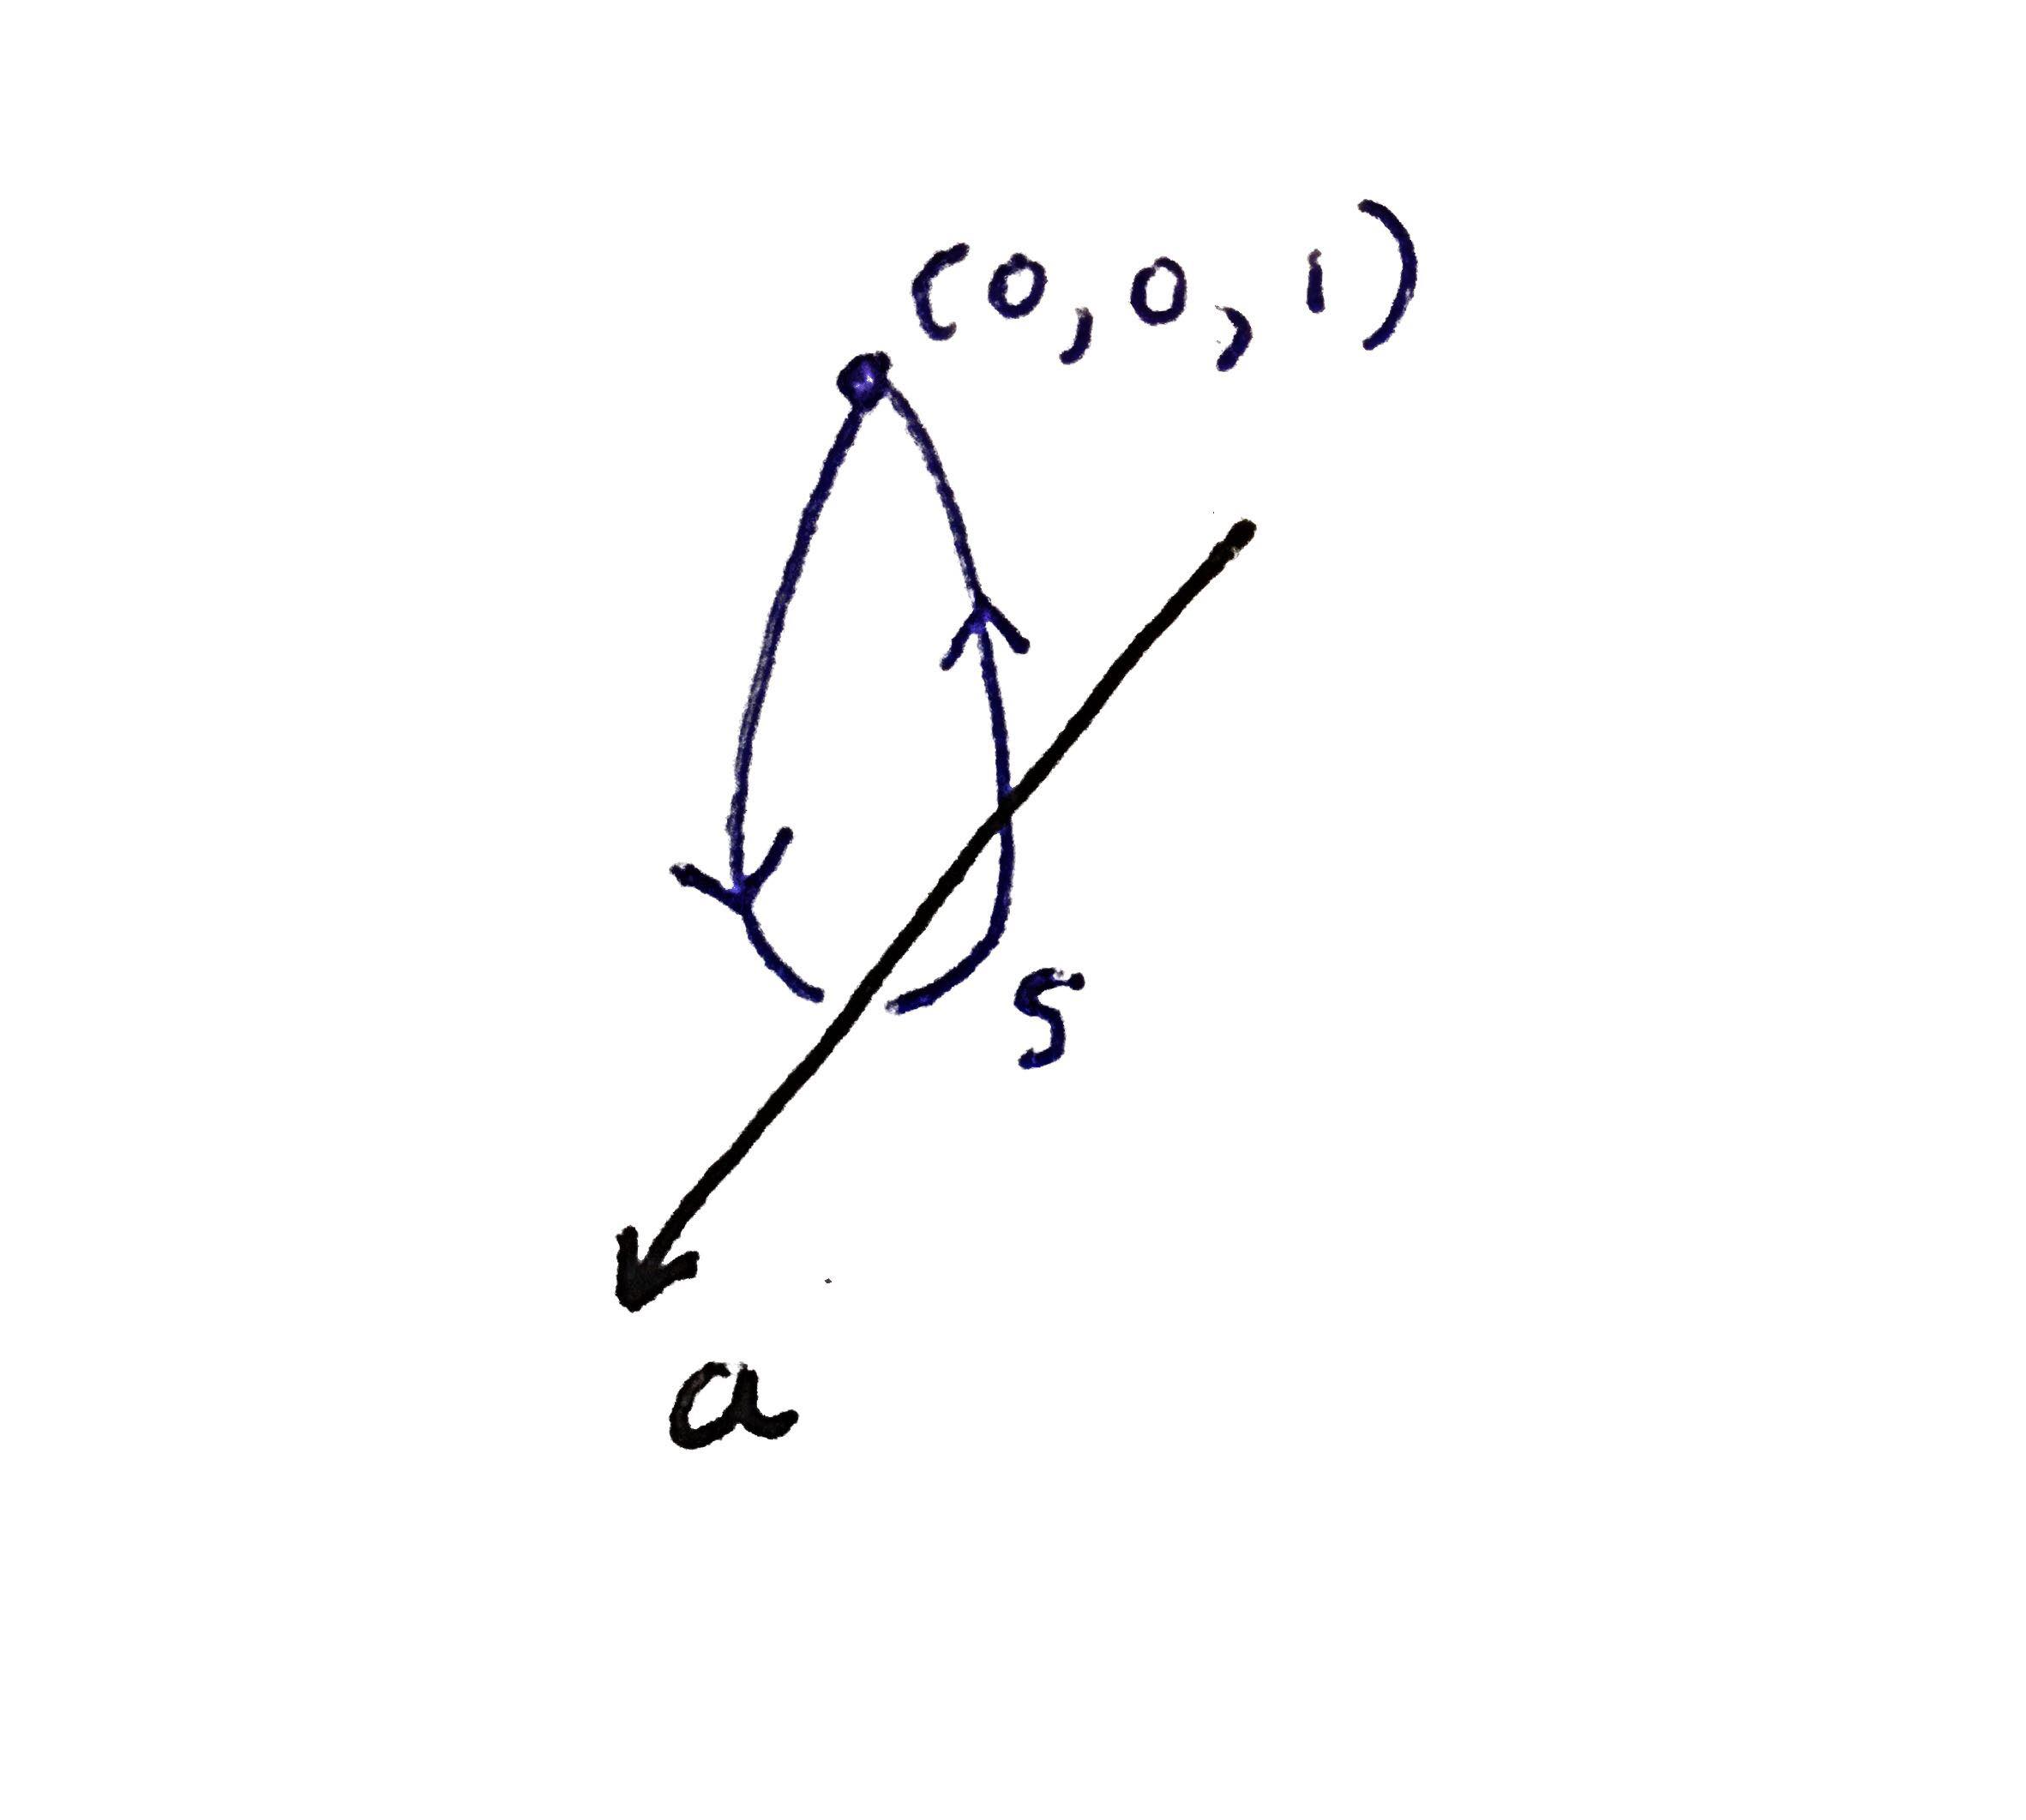
\includegraphics[width=4in]{figures/s_loop.png}
	\caption{Zooming out to see $s$, which begins and ends at the point (0,0,1).}
	\label{fig:rtinstability}
\end{figure}

\noindent Figure 3 illustrates the division of the Trefoil Knot into three arcs with corresponding loops.\\\\

\begin{figure}[h!]
		\centering
		\captionsetup{width=.75\linewidth}
		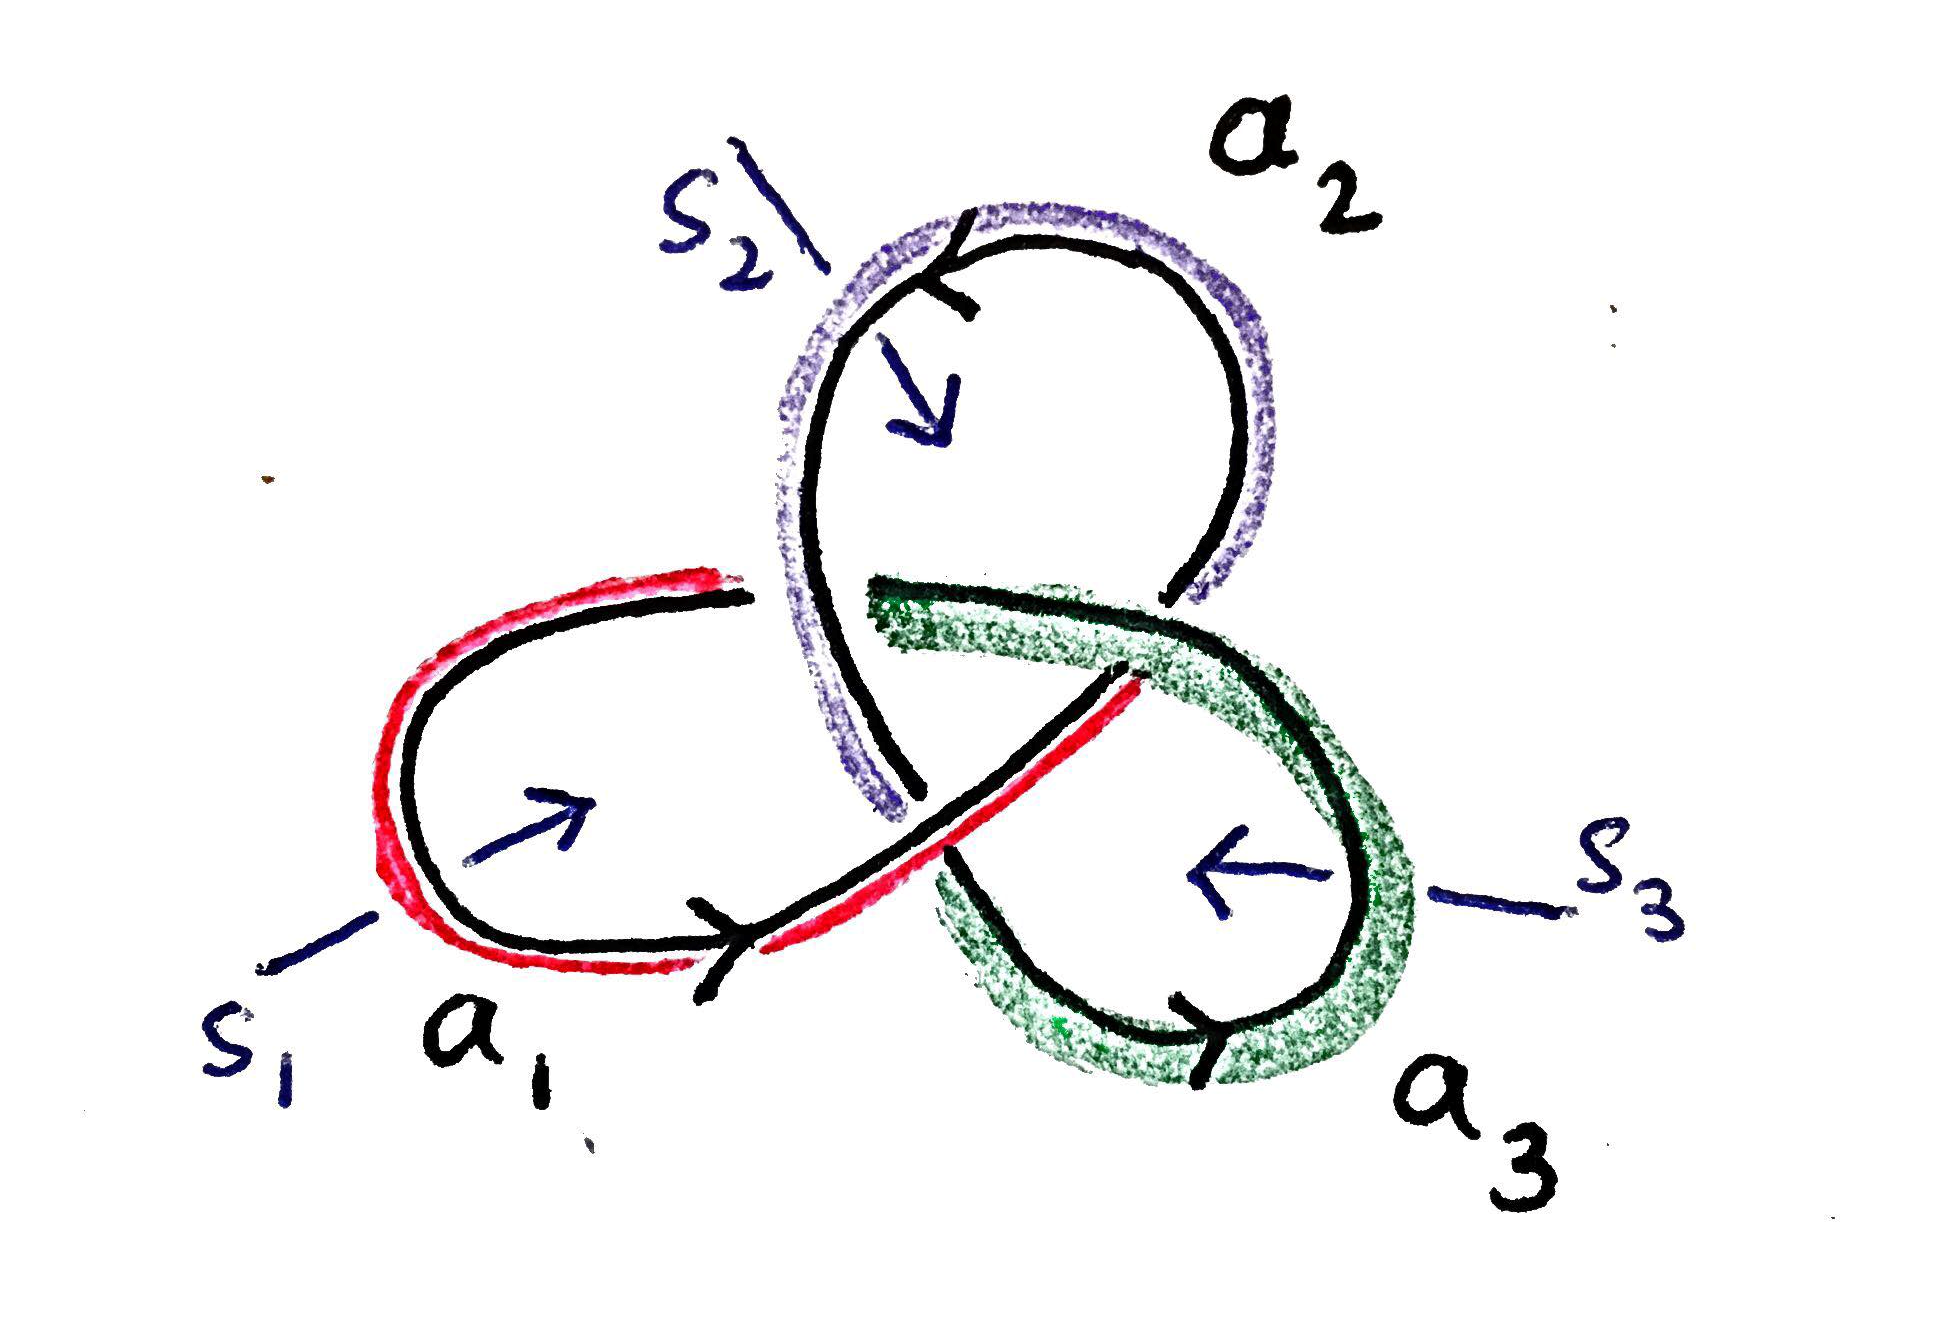
\includegraphics[width=4in]{figures/tref_colors.png}
		\caption{Example: The trefoil knot diagram has three crossings and thus three arcs, colored red, purple, and green respectively. Arrows indicate the knot's direction. Each $s_i$ travels below $a_i$ from right to left.}
		\label{fig:rtinstability}
\end{figure}

\noindent Now we can consider the equivalence classes of loops at a crossing, using our orientation convention. Any crossing in a knot diagram involves three arcs: two for the part of the knot on the bottom of the crossing and one for the part on top. Three distinct loops encircle the arcs. We let $s_i$ be the (equivalence class of the) loop that travels around arc $a_i$. The image in Figure 4 and 5 below shows how loops are oriented at the two types of crossings.

\begin{figure}[h!]
		\centering
		\captionsetup{width=.75\linewidth}
		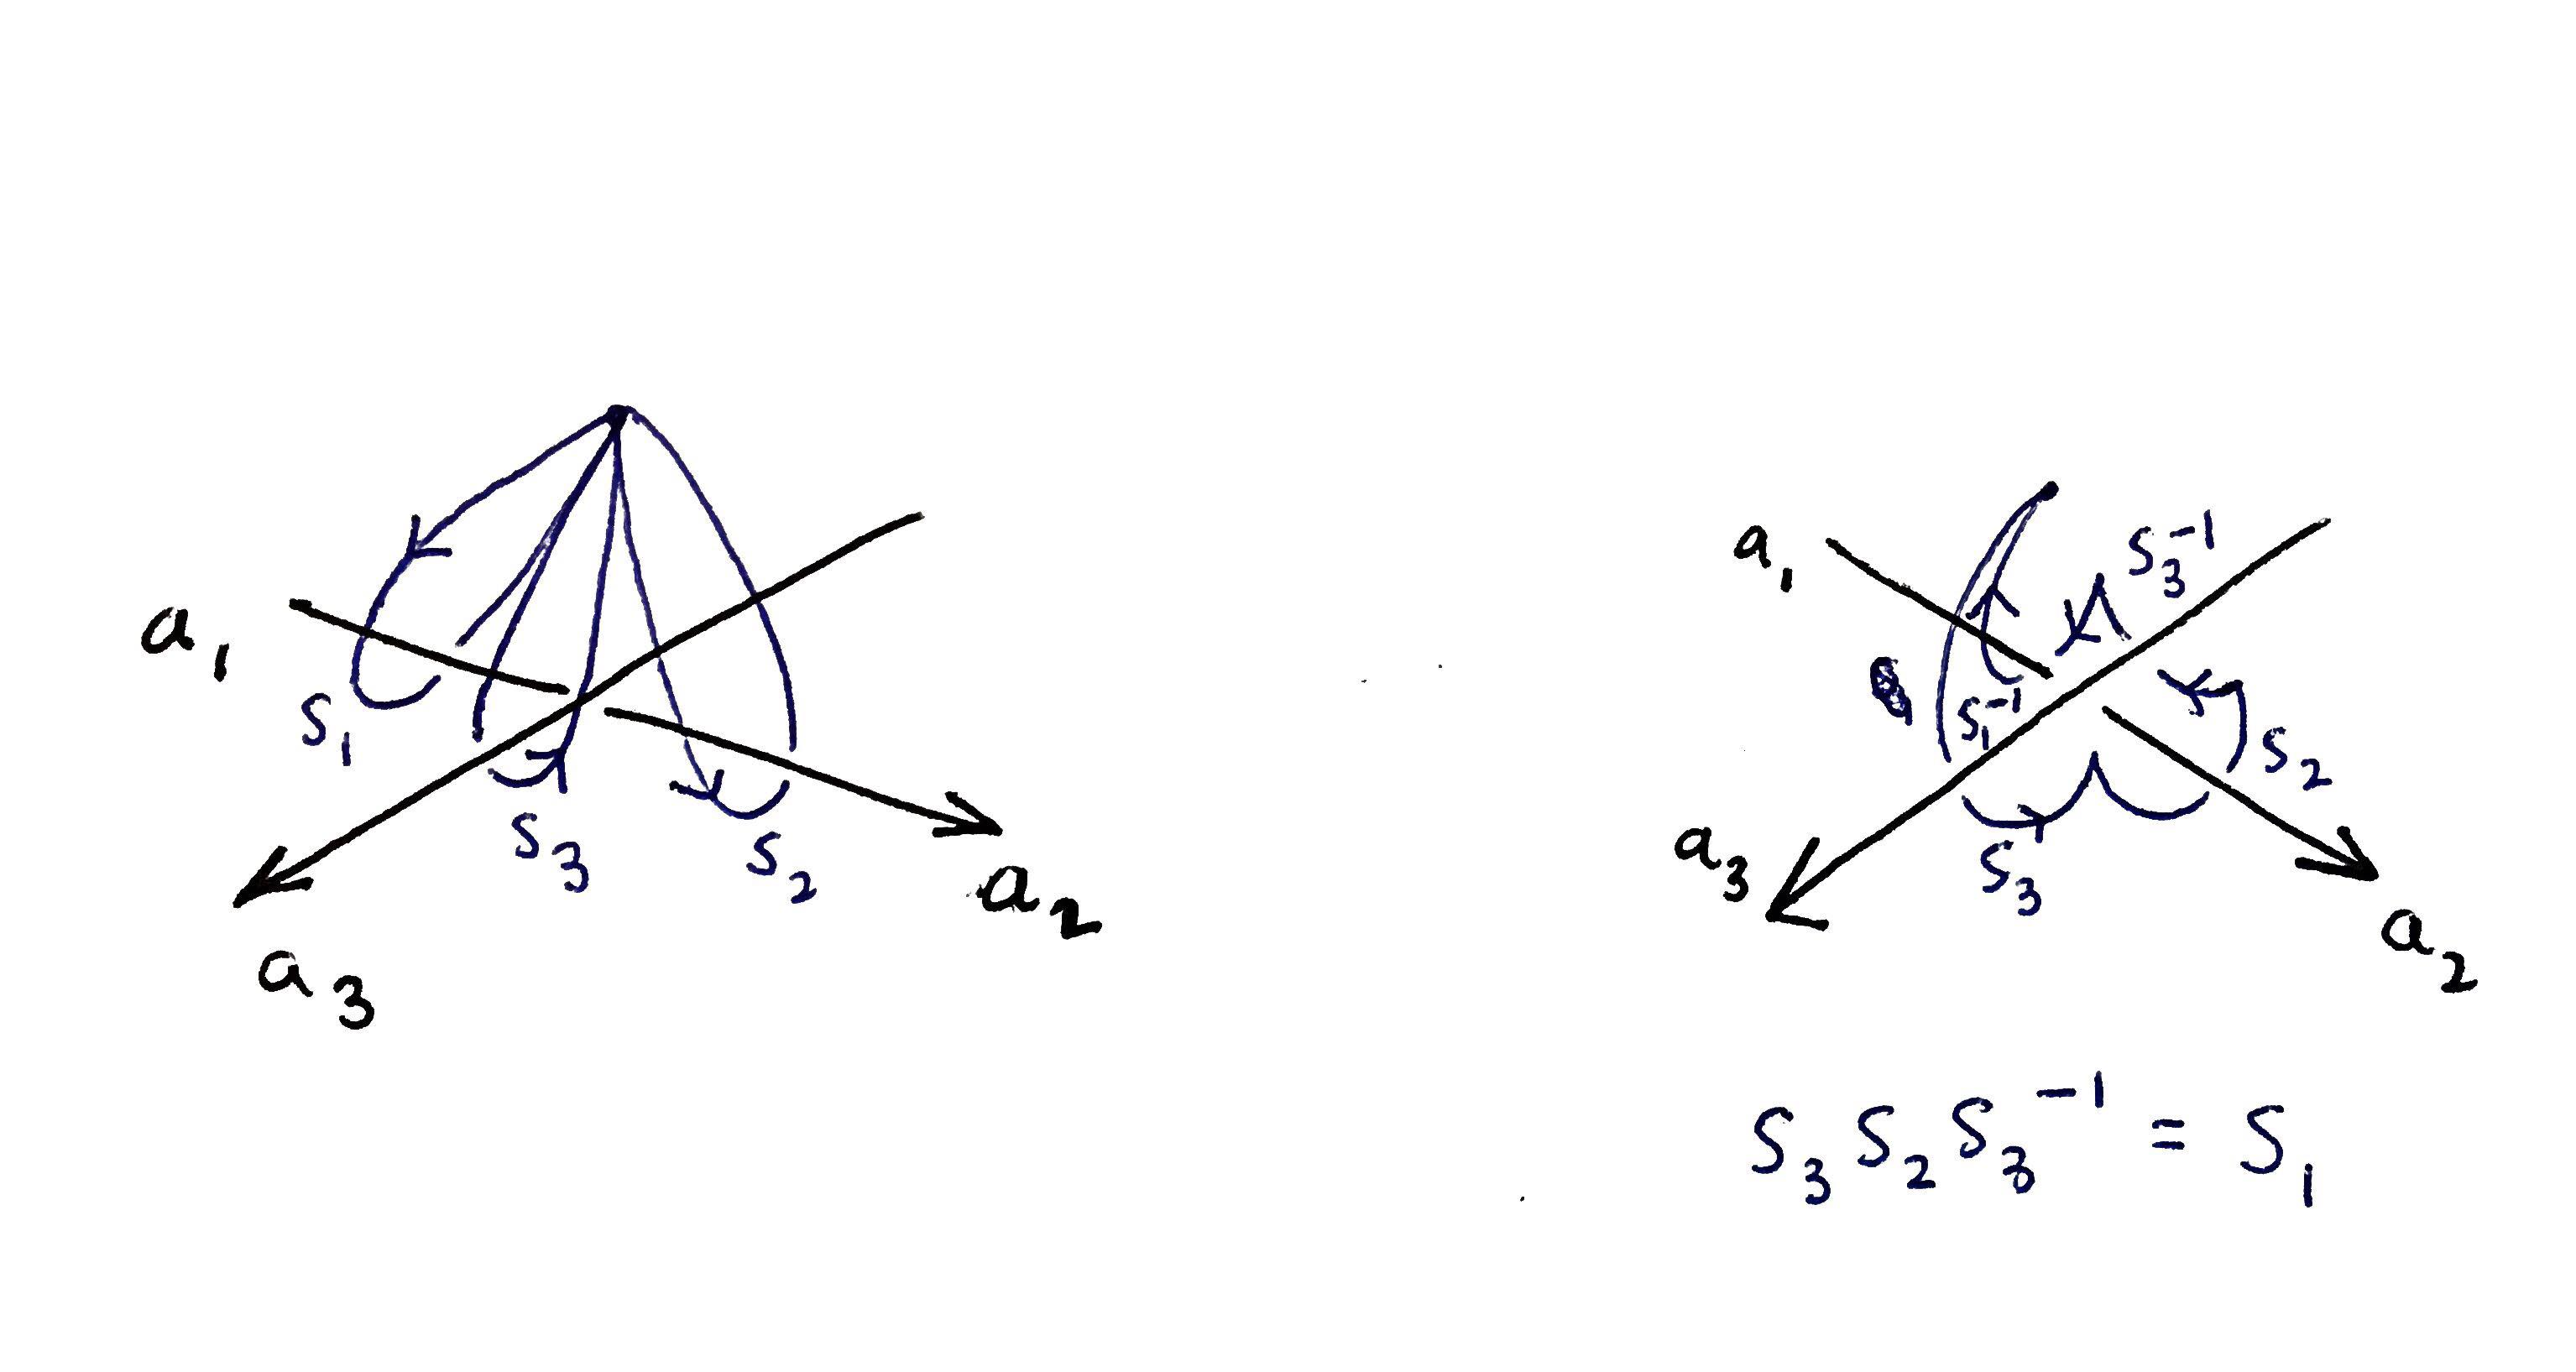
\includegraphics[width=6in]{figures/loops_s1.png}
		\caption{Loops $s1, s2, s3$ at crossing 1. $a_3$ travels towards the bottom left corner of the page. The right hand image demonstrates how to compose the three loops to get a loop that is homotopic to the identity.}
		\label{fig:rtinstability}
	\end{figure}
	
	\begin{figure}[h!]
		\centering
		\captionsetup{width=.75\linewidth}
		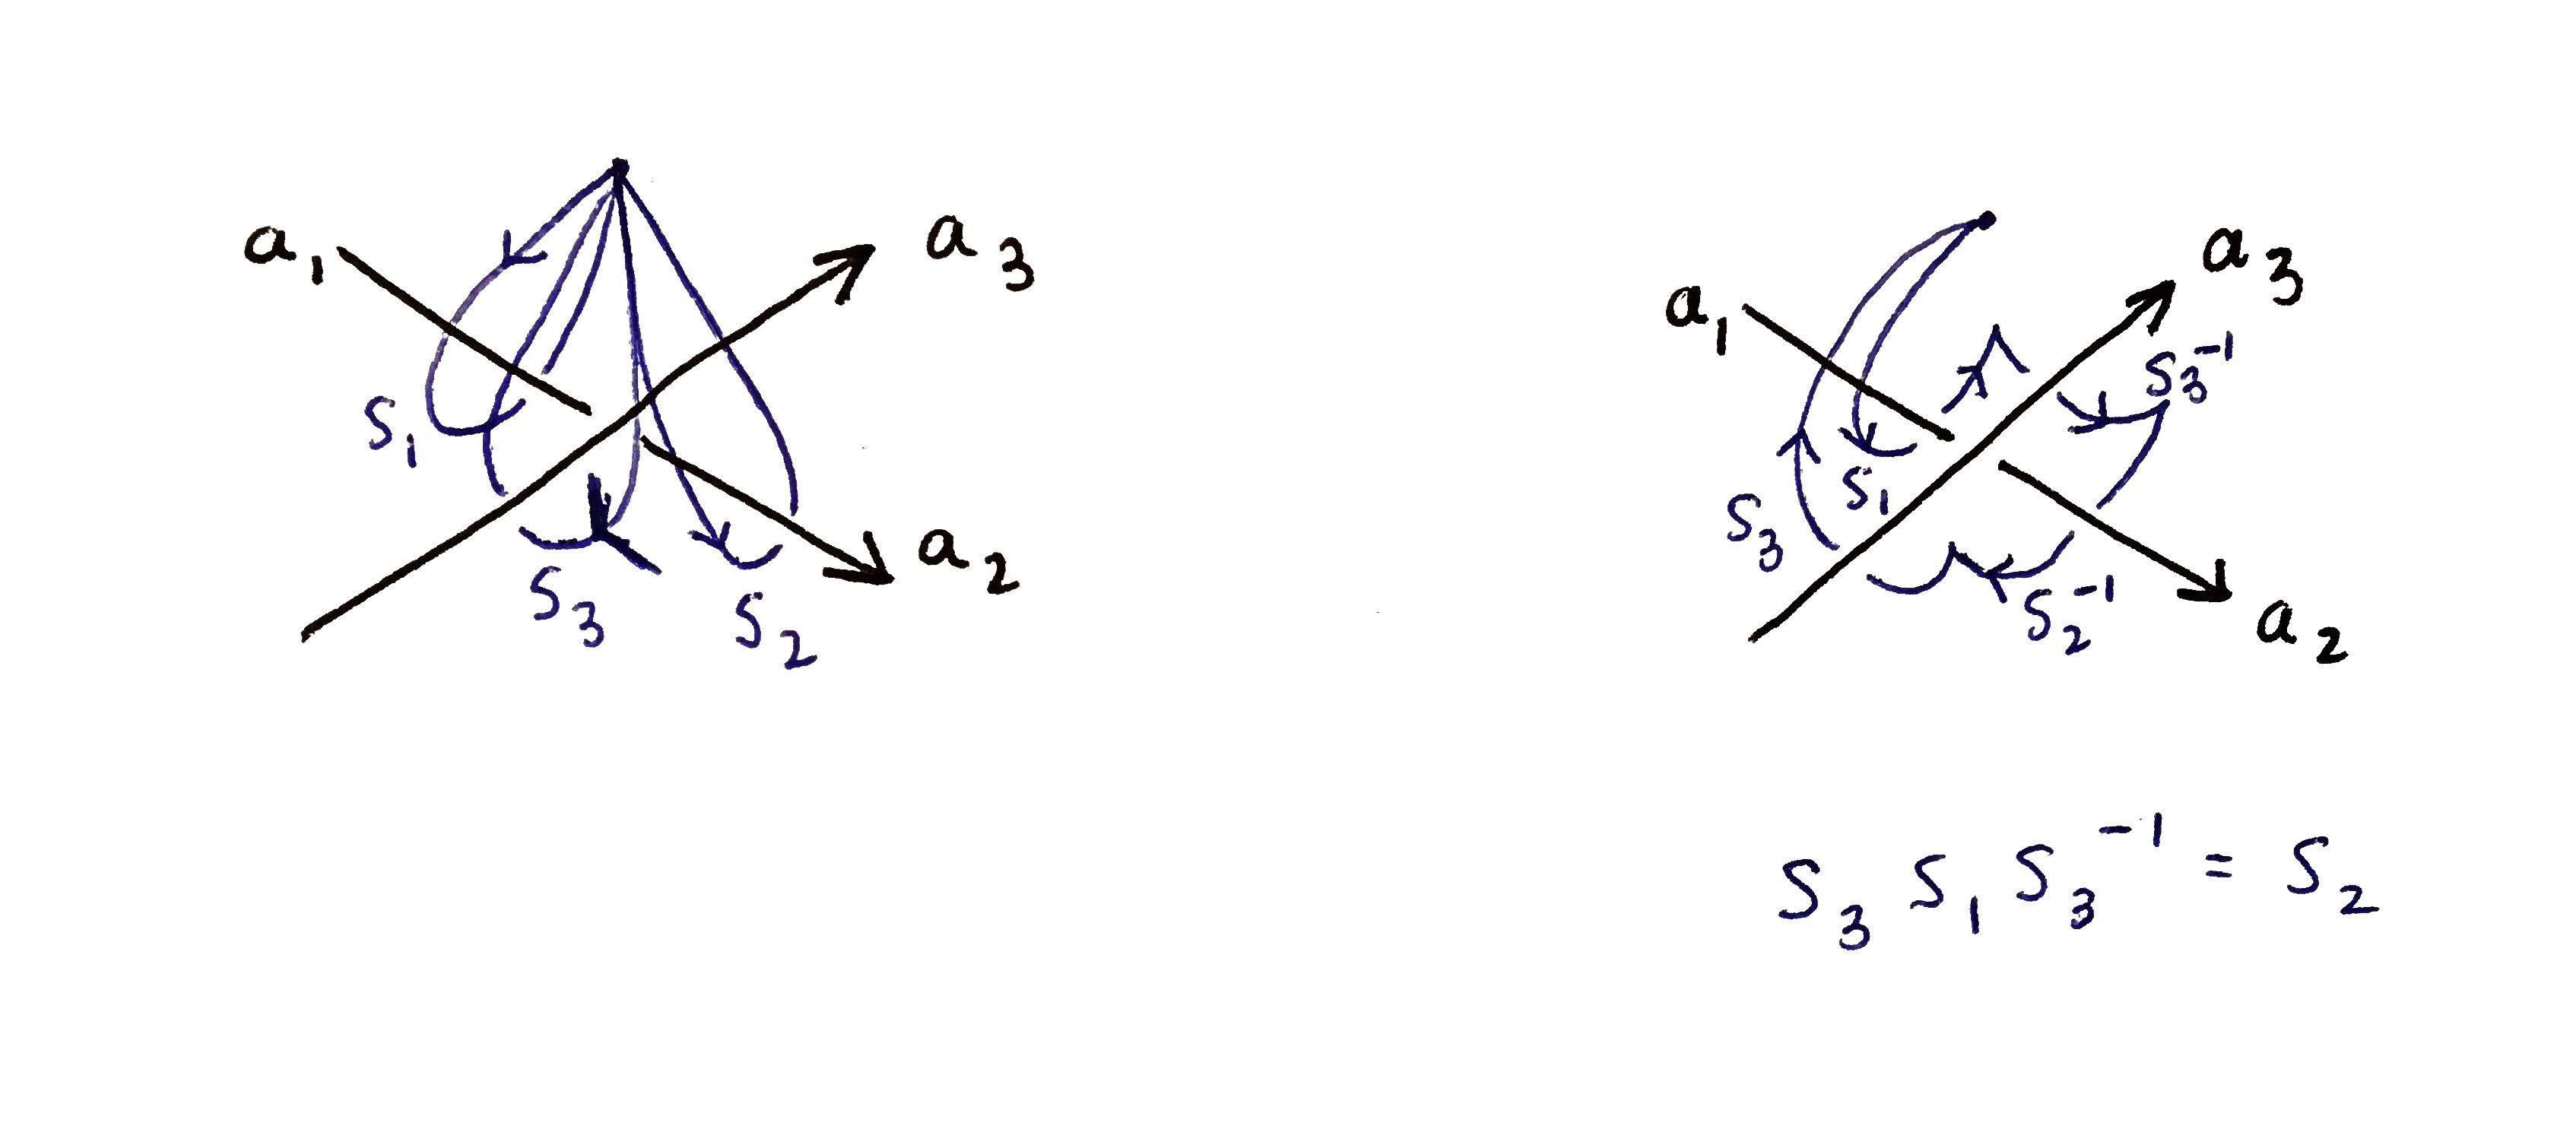
\includegraphics[width=6in]{figures/loops_s2.png}
		\caption{Loops $s1, s2, s3$ at crossing 2. $a_3$ travels towards the upper right corner of the page.}
		\label{fig:rtinstability}
	\end{figure}
\end{definition}	
	
\noindent From the first diagram (Figure 4), we see that composing the loops in the following way gives the relation:
\[s_3s_2s_3^{-1}s_1^{-1} = e\]
And thus
\[s_1 = s_3s_2s_3^{-1}\]
\noindent Similarly, from the second diagram (Figure 5) we get the relation
\[s_1s_3^{-1}s_2^{-1}s_3 = e\]
And so
\[s_2 = s_3s_1s_3^{-1}\]
\noindent In general, for an arbitrary knot diagram with arcs $a_1, ..., a_n$, each of the arcs would have their corresponding $s_1, ..., s_n$. At each crossing from $a_i$ to $a_{(i + 1)\ (mod\ n)}$ with $a_k$ on top, let $j = (i + 1)\ (mod\ n)$, then there are two possible relations.\\\\
Either,
\[s_i = s_k(s_{j})s_k^{-1}\]
Or,
\[s_{j} = s_k(s_i)s_k^{-1}\]
We will refer to the relation that holds as $r_i$.\\\\
It turns out that we can find the knot group of a given knot using $s_i$ and $r_i$.

\begin{claim}[The Wirtinger Presentation]
The equivalence classes of the loops $s_i$ generate the knot group of $K$. This group, $\pi_1(\mathbb{R}^3\setminus K)$, has the following presentation:
\[ \pi_1(\mathbb{R}^3\setminus K) \cong \langle s_1,s_2,...s_n\ |\ r_1,r_2,...r_n \rangle\] 
where $r_i$ is the relation we get between the three loops involved in crossing $i$ in the knot diagram.
\end{claim}

\begin{example}[The Knot Group of a Trefoil]
We observe that in Figure 3, each crossing is the second type of crossing. Crossing 2 is shown in Figure 5. Using Figure 5, we have the following relations from each crossing:

\[r_1: s_3 = s_1s_2s_1^{-1}\]

\[r_2: s_2 = s_3s_1s_3^{-1}\]

\[r_3: s_1 = s_2s_3s_2^{-1}\]

\noindent We obtain the presentation of the knot group of the trefoil:
\[ \langle s_1,s_2,s_3\ |\ s_1s_2s_1^{-1} = s_3,\ s_3s_1s_3^{-1} = s_2,\ s_2s_3s_2^{-1} = s_1\rangle\ \]
\end{example}

\begin{example}[The Knot Group of an Unknot]
An Unknot has just 1 arc $a_1$ with the conjugation relations $s_1s_1s_1^{-1} = s_1$, or equivalently that $s_1 = s_1$, so there's no non-trivial relations.\\\\
Thus, the presentation of the knot group of the unknot is just:
\[\langle s_1\ |\ s_1 = s_1\rangle  = \langle s_1\ |\ \O \rangle = \mathbb{Z}\]
It can be shown that the knot group of the trefoil is not abelian and hence not isomorphic to $\mathbb{Z}$. Thus, the Trefoil and the Unknot are not equivalent knots.
\end{example}

\noindent The {\bf ``Wirtinger Presentation"} gives us a consistent algorithm in calculating the knot group of a given knot. Unsurprisingly, the heart of proving this algorithm lies in the clever application of Van Kampen's Theorem.

\begin{proof}[Proof of Wirtinger Presentation]
For any given knot diagram with $n$ arcs, we will homotope the diagram such that all of the knot is on the $xy$-plane (think of it as the cross section of the knot diagram) except for at each crossing, the lower knot is pulled to $z = -1$ to make a trench that falls below the knot above. This preserves the knot group of the original knot, and we will denote the new figure as $K$.\\\\
Figure 6 below shows an example of what the Trefoil Knot would look like under the transformation we described above:
	\begin{figure}[h!]
		\centering
		\captionsetup{width=.75\linewidth}
		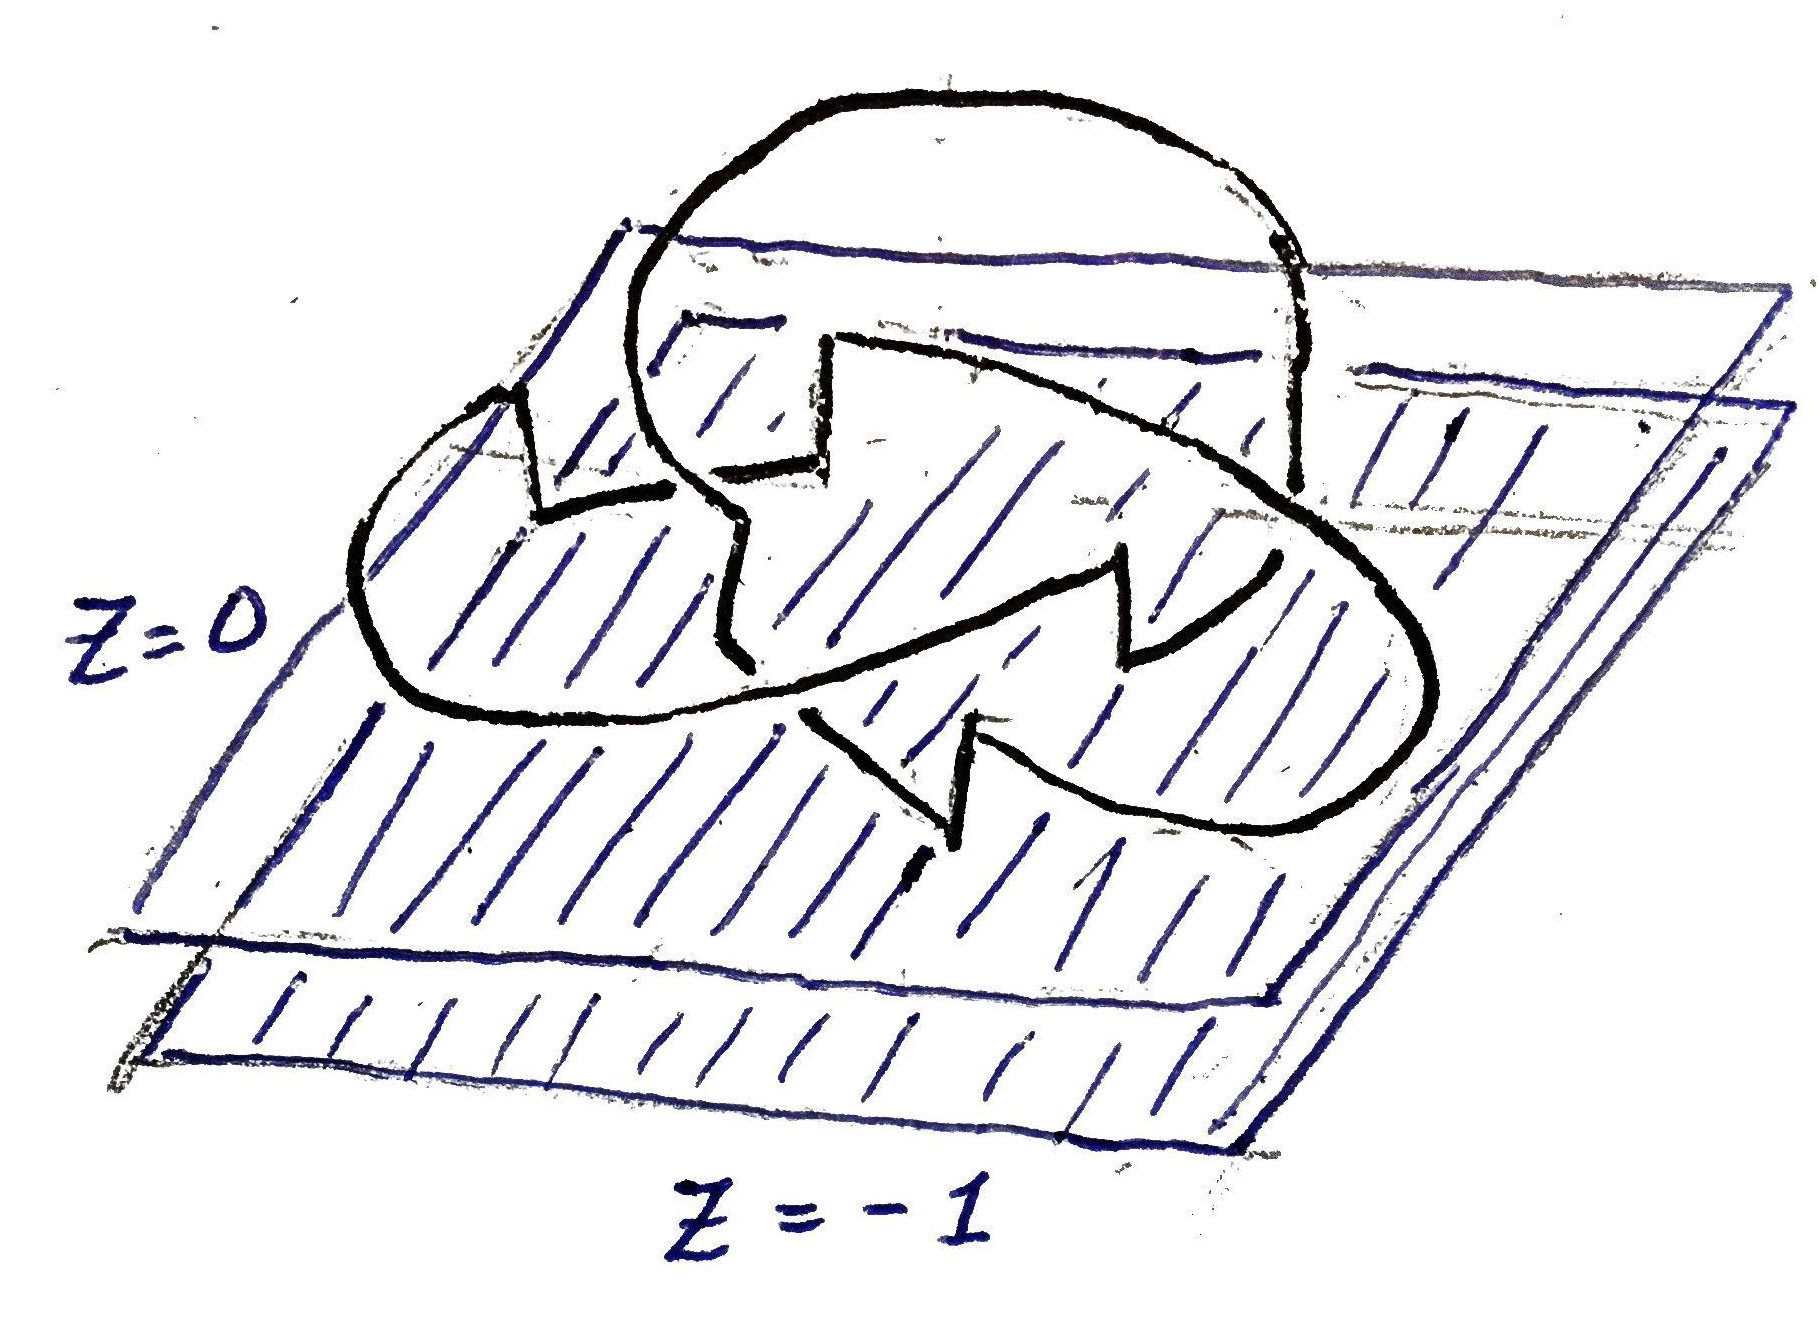
\includegraphics[width=.5\linewidth]{figures/trefoil_crossings.png}
		\caption{This is the Trefoil Knot under our transformation, notice that at each crossing the lower knot falls from $z = 0$ to $z = -1$ to make a ``trench."}
		\label{fig:rtinstability}
	\end{figure}
We will label the trenches $T_1, ..., T_n$, where $T_i$ is the trench formed when the arc $a_{i}$ turns to $a_{i + 1\ (mod\ n)}$.\\\\
Clearly, $\mathbb{R}^3 - K$ is still path-connected, so the base point is irrelevant.\\\\
Let $G = \pi_1(\mathbb{R}^3 - K)$, we will calculate G using Van Kampen's Theorem by appropriately dividing $\mathbb{R}^3 - K$ into a union of open, path-connected subspaces.\\\\
Indeed, let $U = \{(x, y, z) \in \mathbb{R}^3\ |\ z \geq -1\} - K$.\\\\
Let $W_1, ..., W_n$ be a sequence of subspaces where $W_i$ corresponds to a rectangular box under $T_i$ whose ceiling is at $z= -1$ but has $T_i$ removed, and the box is adjoined with an arc to $(0, 0, 1)$, which is the basepoint where the loops we are interested in originate from. The arc can be formed such that it's disjoint from $K$.\\\\
Figure 7 below here shows what $W_i$ would look like:
	\begin{figure}[h!]
		\centering
		\captionsetup{width=.75\linewidth}
		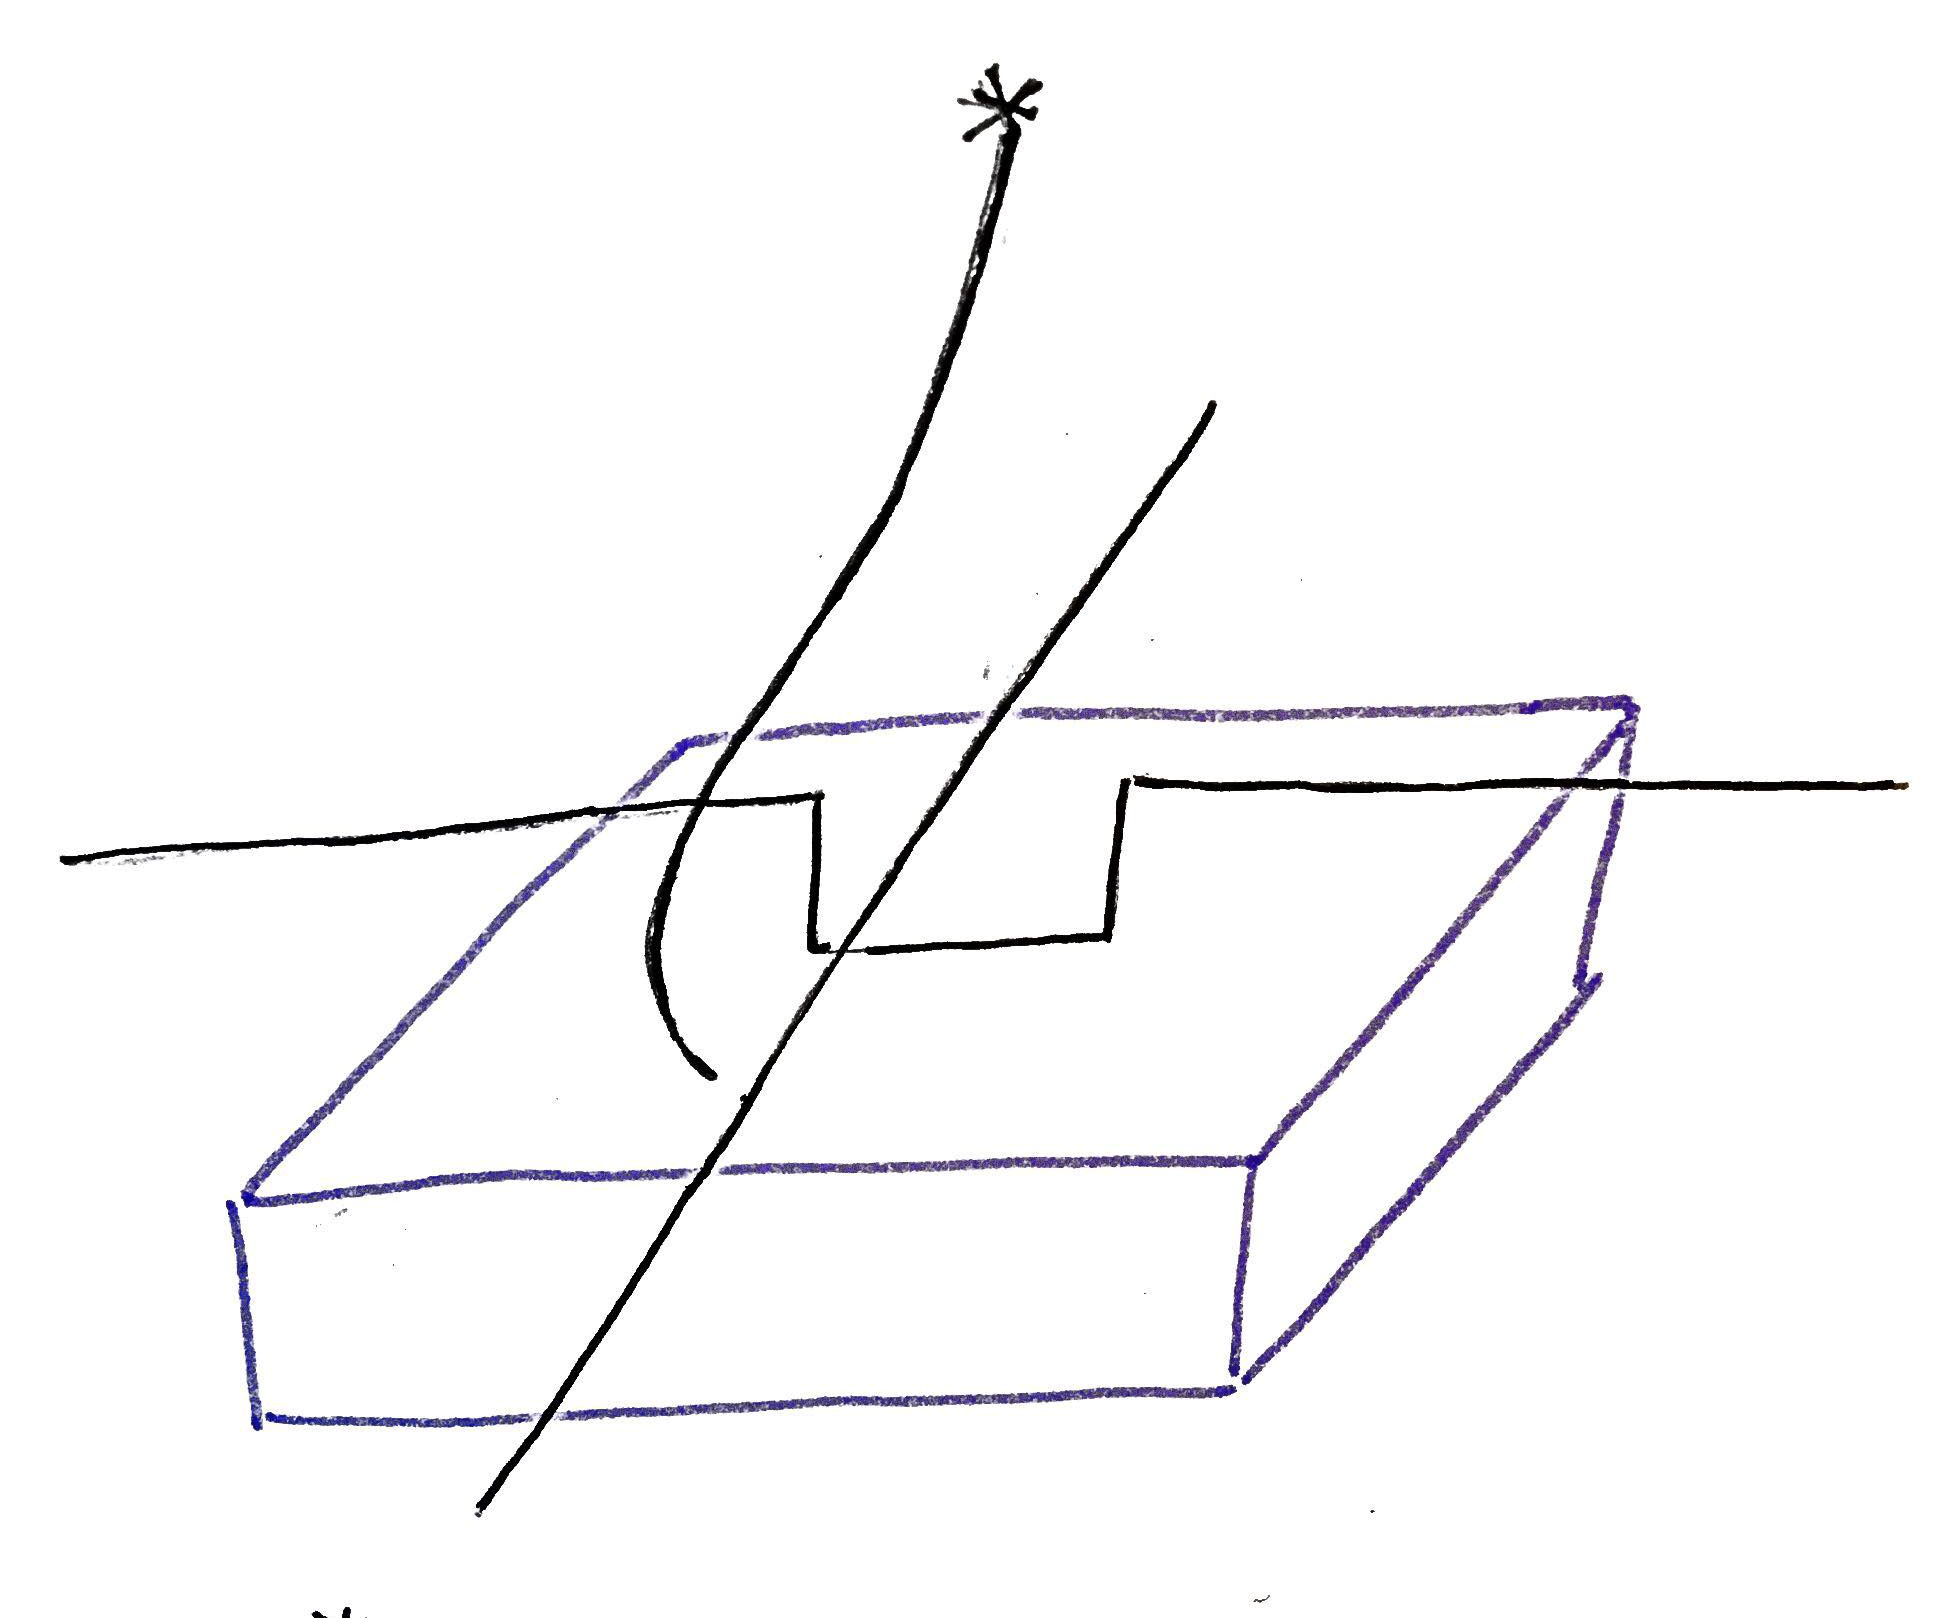
\includegraphics[width=.3\linewidth]{figures/box.png}
		\caption{This is an example of what $W_i$ would look like. Note that the knot is not part of $W_i$}
		\label{fig:rtinstability}
	\end{figure}
We will choose each $W_i$ within $W_1, ..., W_n$ such that they are pairwise disjoint spaces. We can do this by limiting the size of the boxes.\\\\
Let $V = cl(\mathbb{R}^3 - (U \cup W_1 \cup ... W_n))\bigcup A$, where V is the closure of the complement of U and all of $W_i$, adjoined with the set A, which is an arc to $(0, 0, 1)$ such that A is disjoint from K.\\\\
Clearly, $\mathbb{R}^3 - K = U \cup (W_1 \cup  ... \cup W_n) \cup V$, and we will proceed to use Van Kampen's Theorem to calculate $\pi_1(\mathbb{R}^3 - K)$.\\\\
{\bf 1. $\pi_1(U)$ is the free group of rank n:}\\\\
We claim that $\pi_1(U) = \langle s_1, ..., s_n\ | \O\rangle$.\\\\
The idea is that we can partition U up again as n arcs with their ends pinned $z = -1$ such that their intersections are all simply connected, and 1 leftover space that's simply connected and has simply connected intersection with the arc spaces. We will call the n spaces partitioned $X_1, ..., X_n$.\\\\
Then $\pi_1(U)$ is the free product of all $\pi_1(X_i)$, as the amalgamation can be ignored as the intersections are simply connected.\\\\
You can see in Figure 8 an illustration of said space.\\\\
	\begin{figure}[h!]
		\centering
		\captionsetup{width=.75\linewidth}
		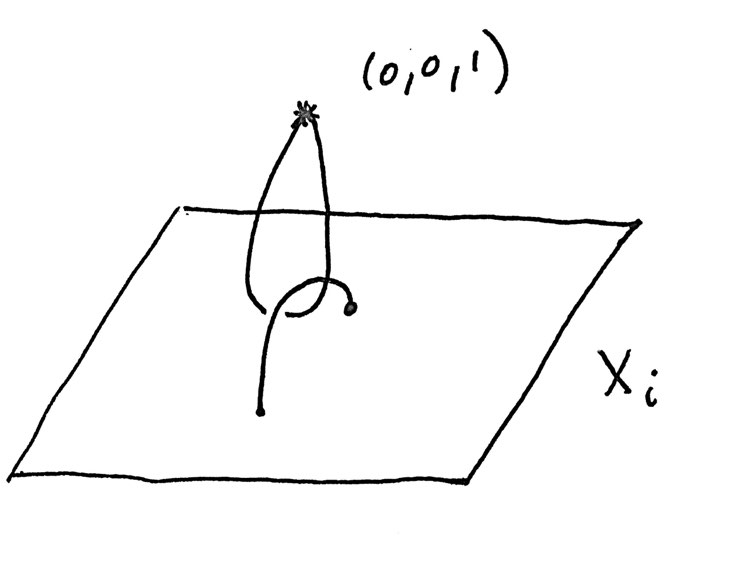
\includegraphics[width=.3\linewidth]{figures/knot_loop.jpg}
		\caption{This is an example of what $X_i$ would look like.}
		\label{fig:rtinstability}
	\end{figure}

\noindent For any loop that's outside of the arc (the arc does not cross the loop), they can be homotoped to the constant loop. And for a given loop from basepoint $(0, 0, 1)$ that crosses the arc, which is just $s_i$, we can see that it generates the entire fundamental group.\\\\
Thus, $\pi_1(X_i) = \langle s_i\ |\ \O\rangle$.\\\\
Since $\pi_1(U)$ is the free product of n free groups of rank 1, we have that:
\[\pi_1(U) = \langle s_1, ..., s_n\ |\ \O \rangle\]
{\bf 2. Combining $W_1$ to U:}\\\\
First we will start with $W_1$, then the rest of $W_2, ..., W_n$ follows similarly.\\\\
Let $i: U \bigcap W_1 \to U$, $j: U \bigcap W_1 \to W_1$ be the two inclusion maps.\\\\
By Van Kampen, we know that $\pi_1(U \bigcup W_1)$ is the free product of $\pi_1(U)$ and $\pi_1(W_1)$ with amalgamation $\pi_1(U \bigcap W_1)$ along with the homomorphism $i_*$, $j_*$.\\\\
$W_1$ itself is clearly simply connected since it deformation retracts to a convex subset of $\mathbb{R}^3$.\\\\
However, $A \bigcap W_1$ deformation retracts to a punctured plane (as illustrated in Figure 9):
	\begin{figure}[h!]
		\centering
		\captionsetup{width=.75\linewidth}
		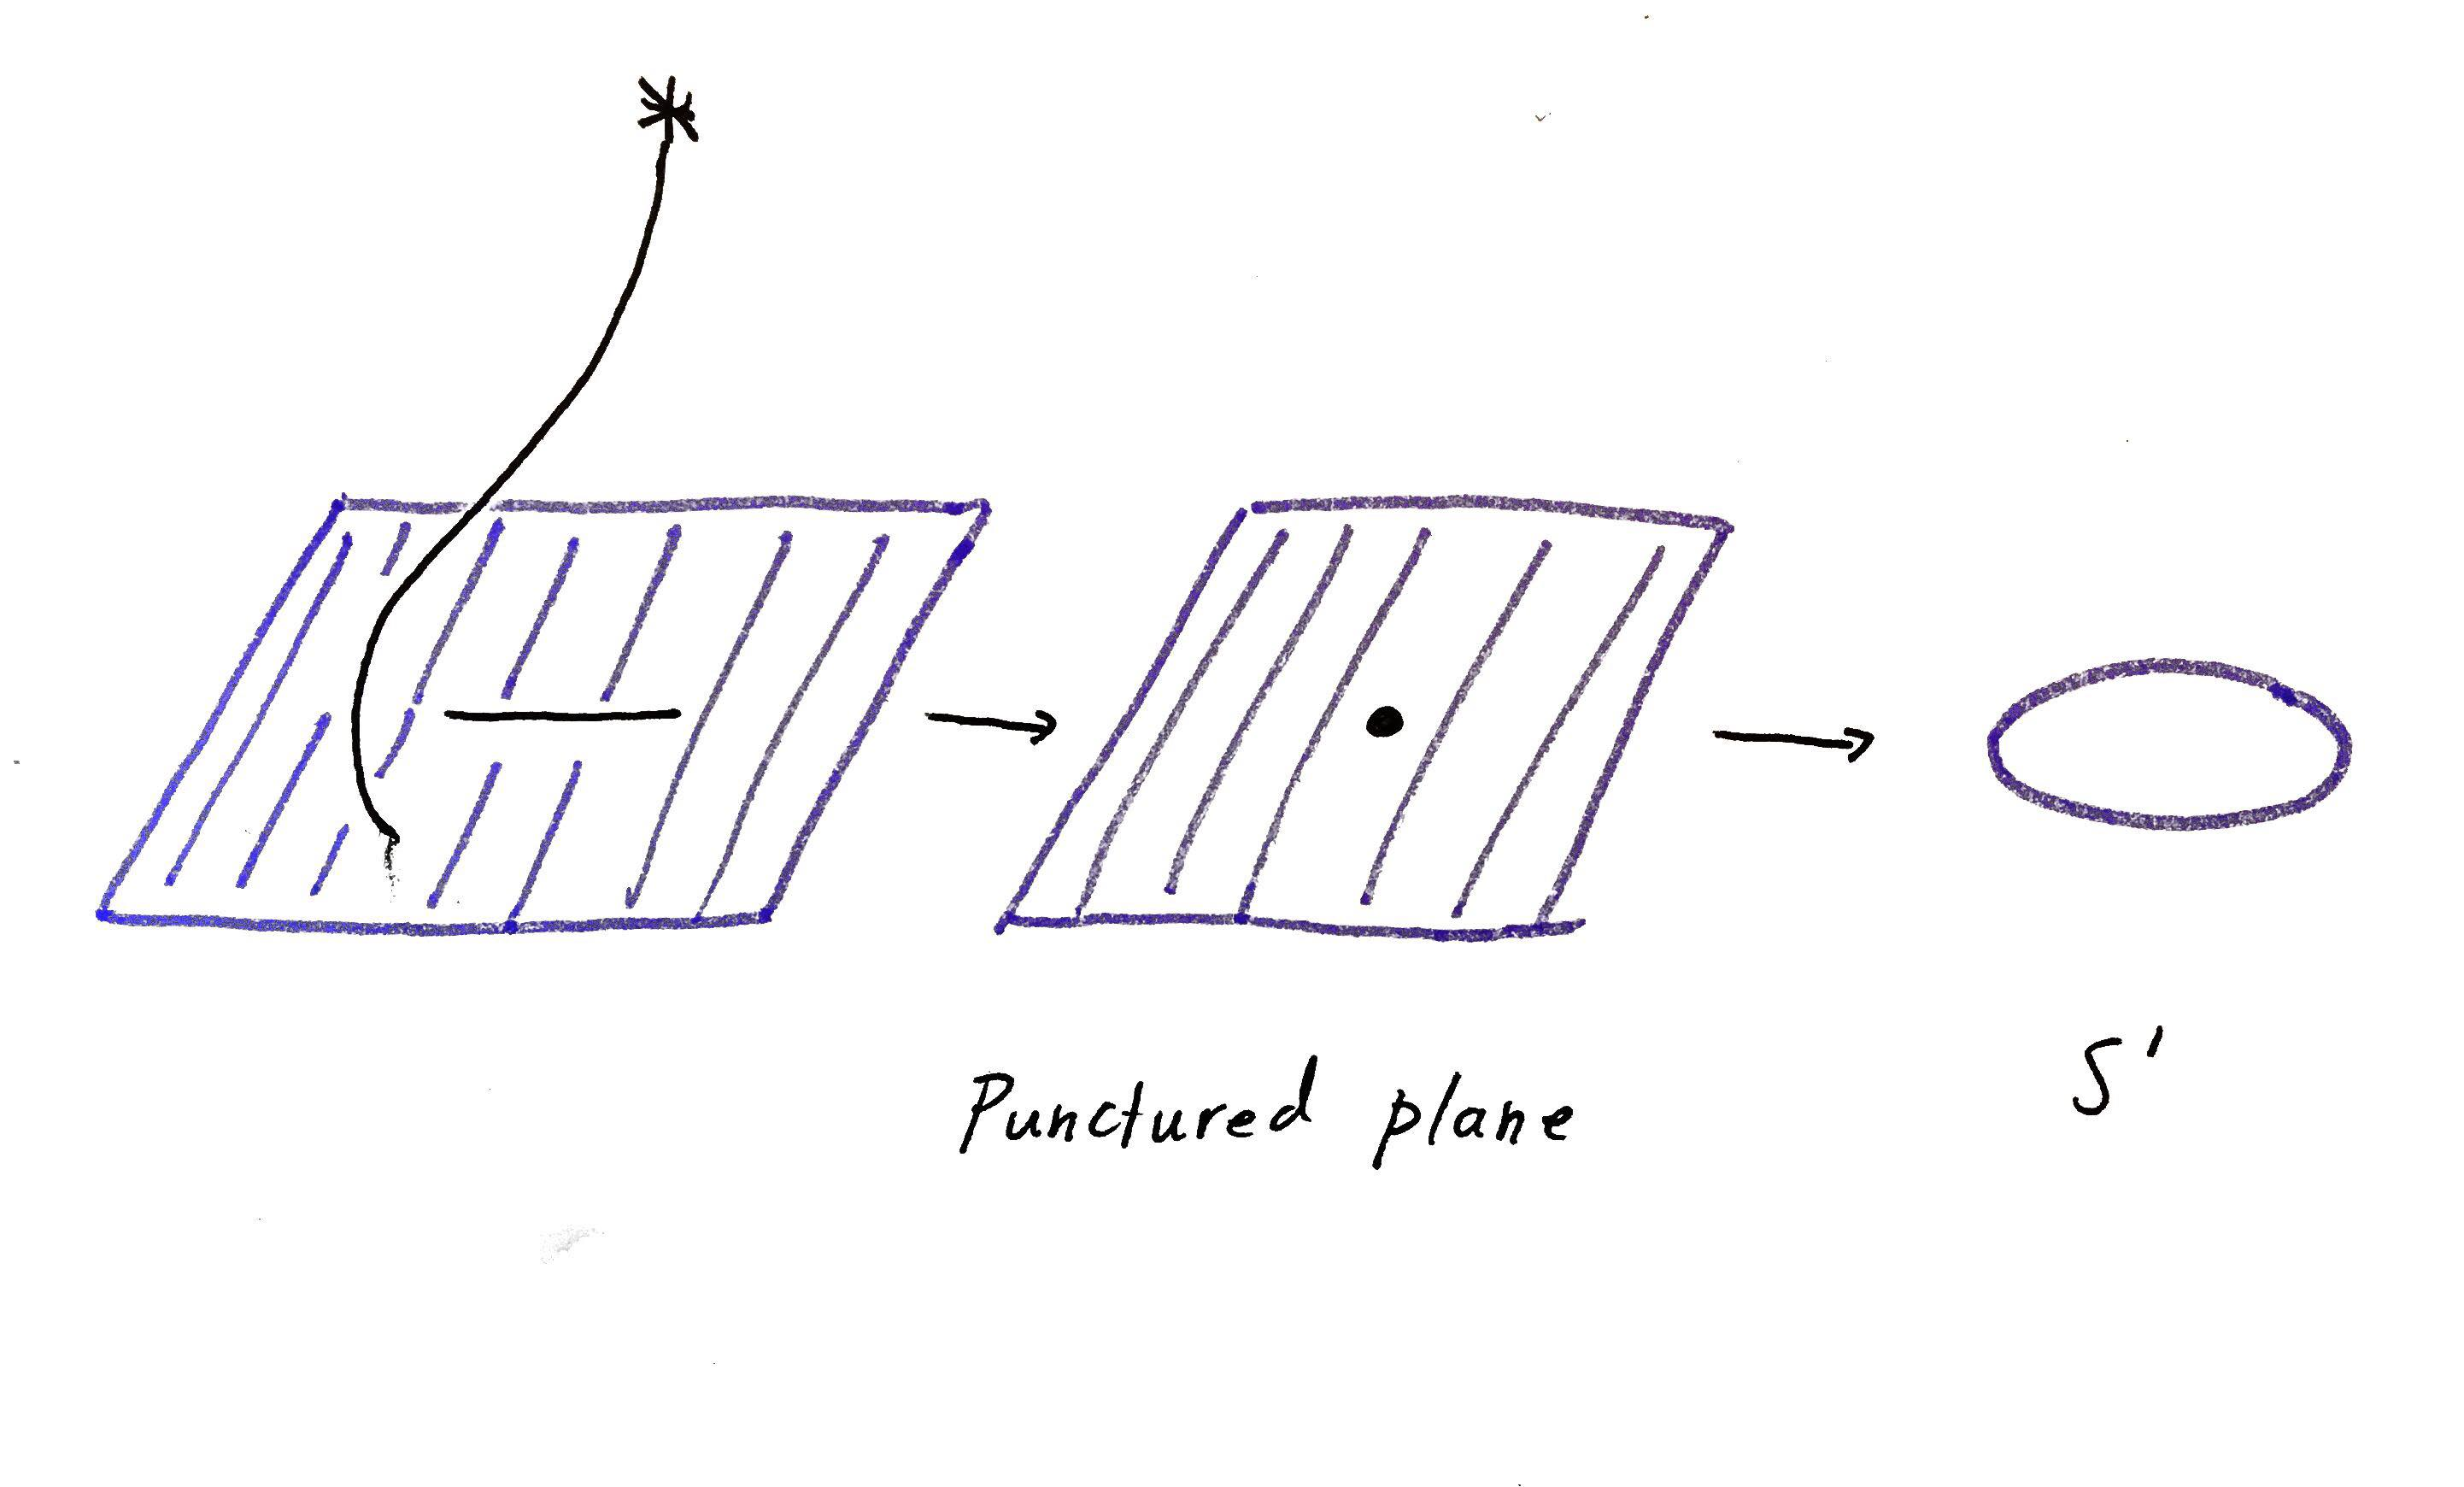
\includegraphics[width=4in]{figures/def_retr.jpg}
		\caption{This Figure illustrates the deformation retraction of $U \bigcap W_1$}
		\label{fig:rtinstability}
	\end{figure}
Therefore $\pi_1(U \bigcap W_1)$ is the free group of rank 1, and we will denote it as $\pi_1(U \bigcap W_1) = \langle x |\O \rangle$.\\\\
Since $W_1$ is simply connected, x is just going to be mapped to the identity by the induced homomorphism.\\\\
When the generator x in $U \bigcap W_1$ is included into U, however, it has to either become one of the two relations described in the theorem. The following diagram in Figure 10 illustrates the process:
	\begin{figure}[h!]
		\centering
		\captionsetup{width=.75\linewidth}
		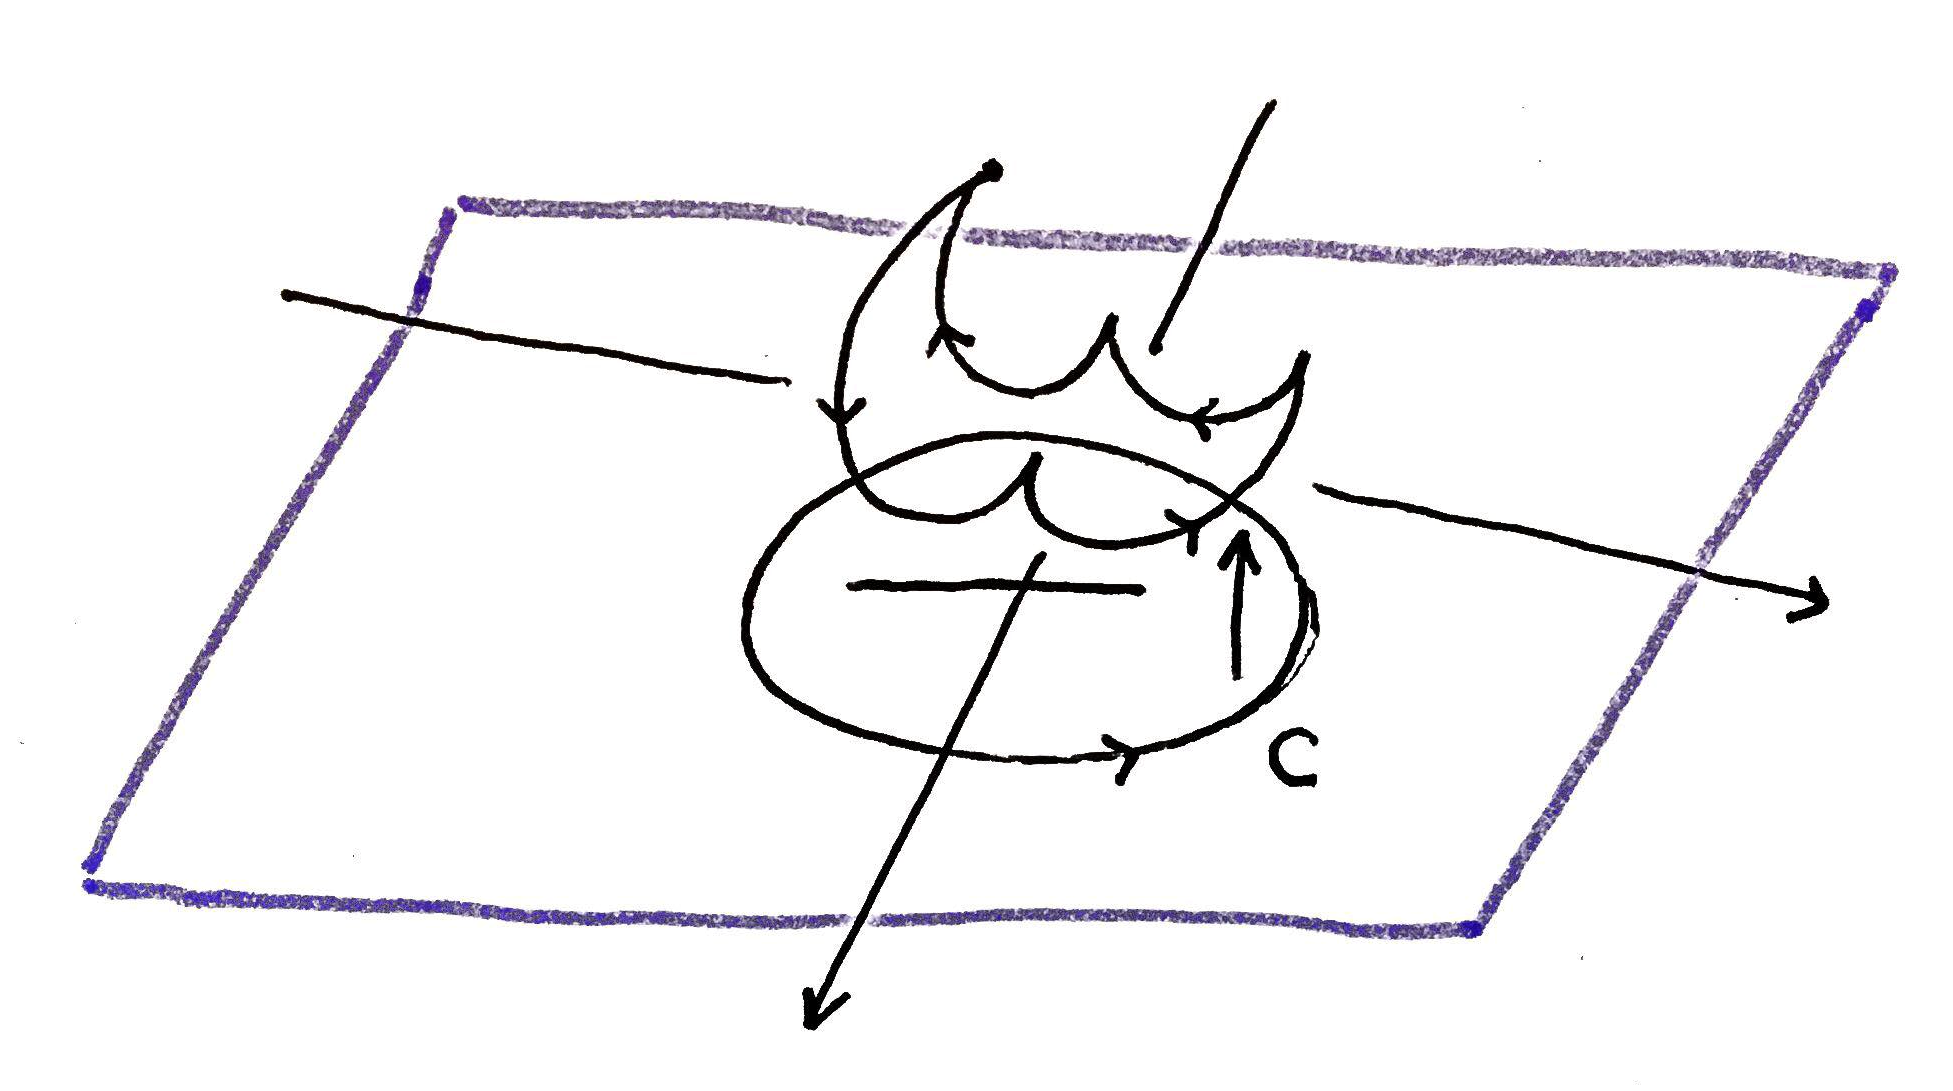
\includegraphics[width=4in]{figures/loop_above_plane.png}
		\caption{We can see in this figure that the circle C when included in U can become the loop above.}
		\label{fig:rtinstability}
	\end{figure}
Without the loss of generality, we say that for the induced homomorphism $i_*: \pi_1(U \bigcap W_1) \to \pi_1(U)$, $i_*(x) = s_ks_2s_k^{-1}s_1^{-1}$.\\\\
Therefore, by Van Kampen's Theorem we know that:
\[\pi_1(U \cup W_1) = \langle s_1, ..., s_n\ |\ i_*(x)j_*(x)\rangle = \langle s_1, ..., s_n\ |\ s_ks_2s_k^{-1}s_1^{-1} = e\rangle = \langle s_1, ..., s_n\ |\ r_1\rangle\]
{\bf 3. Combining $W_2, ..., W_n$ to $U \bigcup W_1$:}\\\\
The process for $\pi_1(A \cup W_1)$ and $\pi_1(W_2)$ is nearly identical since $W_2$ is simply connected, and $W_1$ and $W_2$ are disjoint, so $\pi_1(A \cup W_1 \cap W_2) = \mathbb{Z}$, and everything else follows similarly.\\\\
So we have that:
\[\pi_1(U \cup W_1 \cup W_2) = \langle s_1, ..., s_n\ |\ r_1, r_2\rangle\]
And thus everything up to $S_n$ also follows similarly, so
\[\pi_1(U \cup W_1 \cup ... W_n) = \langle s_1, ..., s_n\ |\ r_1, ..., r_n\rangle\]
{\bf 4. Combining $V$ to $U \cup W_1 \cup ... W_n$}\\\\
Clearly, V itself is simply connected since it deformation retracts to a convex subset of $\mathbb{R}^3$, and $(U \cup W_1 \cup ... W_n) \bigcap V$ is also simply connected. Therefore, combining V has no effect on the fundamental group, so:
\[\pi_1(U \cup W_1 \cup ... W_n \cup V) = \langle s_1, ..., s_n\ |\ r_1, ..., r_n\rangle\]
{\bf 5. Finishing the Proof:}\\\\
Thus, we have that:
\[\pi_1(\mathbb{R}^3 - K) = \pi_1(U \cup W_1 \cup ... W_n \cup V) = \langle s_1, ..., s_n\ |\ r_1, ..., r_n\rangle\]
\end{proof}

\newpage
\section{Conclusion}
We have investigated how to distinguish knots using knot groups and techniques in Algebraic Topology. Van Kampen's Theorem related the fundamental group of a space to the fundamental groups of open subspaces via free product of amalgamation. Furthermore, the Wirtinger Presentation, whose proof also employed Van Kampen's theorem, allowed us to find the knot group of any knot diagram.\\\\
However, there are still some flaws in Wirtinger Presentation itself. It's often not obvious what a given group presentation should be, and simplifying them could prove to be troublesome. However, if the reader is interested in further readings, techniques such as Tietze transformations have been invented to simplify group presentations.\\\\
Nevertheless, the Wirtinger Presentation itself serves as an elegant example at the heart of intersection between Algebraic Topology and Knot Theory, and it reinforces many unique insights Algebraic Topology helps to uncover in the most seemingly distant parts of mathematics.


% bibliography style is set to SIAM here. you can experiment with other styles
\bibliographystyle{siam}

% this line includes all references cited in the document. 
\bibliography{references.bib}
 
\end{document}
